\documentclass{article}

\usepackage{arxiv}

\usepackage[utf8]{inputenc} % allow utf-8 input
\usepackage[T1]{fontenc}    % use 8-bit T1 fonts
\usepackage{lmodern}        % https://github.com/rstudio/rticles/issues/343
\usepackage{hyperref}       % hyperlinks
\usepackage{url}            % simple URL typesetting
\usepackage{booktabs}       % professional-quality tables
\usepackage{amsfonts}       % blackboard math symbols
\usepackage{nicefrac}       % compact symbols for 1/2, etc.
\usepackage{microtype}      % microtypography
\usepackage{graphicx}

\title{spmodel: Spatial Modeling in \textbf{R} -- Computatinal Details Vignette}

\author{
    Michael Dumelle
    \thanks{Corresponding Author}
   \\
    United States \\
    Environmental Protection Agency \\
  200 SW 35th St, Corvallis, OR, 97333 \\
  \texttt{\href{mailto:Dumelle.Michael@epa.gov}{\nolinkurl{Dumelle.Michael@epa.gov}}} \\
   \And
    Matt Higham
   \\
    Department of Math, Computer Science, and Statistics \\
    St.~Lawrence University \\
  23 Romoda Drive, Canton, NY, 13617 \\
  \texttt{\href{mailto:mhigham@stlawu.edu}{\nolinkurl{mhigham@stlawu.edu}}} \\
   \And
    Jay M. Ver Hoef
   \\
    National Oceanic and Atmospheric Administration \\
    Alaska Fisheries Science Center \\
  Marine Mammal Laboratory, Seattle, WA, 98115 \\
  \texttt{\href{mailto:jay.verhoef@noaa.gov}{\nolinkurl{jay.verhoef@noaa.gov}}} \\
  }

% Pandoc syntax highlighting
\usepackage{color}
\usepackage{fancyvrb}
\newcommand{\VerbBar}{|}
\newcommand{\VERB}{\Verb[commandchars=\\\{\}]}
\DefineVerbatimEnvironment{Highlighting}{Verbatim}{commandchars=\\\{\}}
% Add ',fontsize=\small' for more characters per line
\usepackage{framed}
\definecolor{shadecolor}{RGB}{248,248,248}
\newenvironment{Shaded}{\begin{snugshade}}{\end{snugshade}}
\newcommand{\AlertTok}[1]{\textcolor[rgb]{0.94,0.16,0.16}{#1}}
\newcommand{\AnnotationTok}[1]{\textcolor[rgb]{0.56,0.35,0.01}{\textbf{\textit{#1}}}}
\newcommand{\AttributeTok}[1]{\textcolor[rgb]{0.77,0.63,0.00}{#1}}
\newcommand{\BaseNTok}[1]{\textcolor[rgb]{0.00,0.00,0.81}{#1}}
\newcommand{\BuiltInTok}[1]{#1}
\newcommand{\CharTok}[1]{\textcolor[rgb]{0.31,0.60,0.02}{#1}}
\newcommand{\CommentTok}[1]{\textcolor[rgb]{0.56,0.35,0.01}{\textit{#1}}}
\newcommand{\CommentVarTok}[1]{\textcolor[rgb]{0.56,0.35,0.01}{\textbf{\textit{#1}}}}
\newcommand{\ConstantTok}[1]{\textcolor[rgb]{0.00,0.00,0.00}{#1}}
\newcommand{\ControlFlowTok}[1]{\textcolor[rgb]{0.13,0.29,0.53}{\textbf{#1}}}
\newcommand{\DataTypeTok}[1]{\textcolor[rgb]{0.13,0.29,0.53}{#1}}
\newcommand{\DecValTok}[1]{\textcolor[rgb]{0.00,0.00,0.81}{#1}}
\newcommand{\DocumentationTok}[1]{\textcolor[rgb]{0.56,0.35,0.01}{\textbf{\textit{#1}}}}
\newcommand{\ErrorTok}[1]{\textcolor[rgb]{0.64,0.00,0.00}{\textbf{#1}}}
\newcommand{\ExtensionTok}[1]{#1}
\newcommand{\FloatTok}[1]{\textcolor[rgb]{0.00,0.00,0.81}{#1}}
\newcommand{\FunctionTok}[1]{\textcolor[rgb]{0.00,0.00,0.00}{#1}}
\newcommand{\ImportTok}[1]{#1}
\newcommand{\InformationTok}[1]{\textcolor[rgb]{0.56,0.35,0.01}{\textbf{\textit{#1}}}}
\newcommand{\KeywordTok}[1]{\textcolor[rgb]{0.13,0.29,0.53}{\textbf{#1}}}
\newcommand{\NormalTok}[1]{#1}
\newcommand{\OperatorTok}[1]{\textcolor[rgb]{0.81,0.36,0.00}{\textbf{#1}}}
\newcommand{\OtherTok}[1]{\textcolor[rgb]{0.56,0.35,0.01}{#1}}
\newcommand{\PreprocessorTok}[1]{\textcolor[rgb]{0.56,0.35,0.01}{\textit{#1}}}
\newcommand{\RegionMarkerTok}[1]{#1}
\newcommand{\SpecialCharTok}[1]{\textcolor[rgb]{0.00,0.00,0.00}{#1}}
\newcommand{\SpecialStringTok}[1]{\textcolor[rgb]{0.31,0.60,0.02}{#1}}
\newcommand{\StringTok}[1]{\textcolor[rgb]{0.31,0.60,0.02}{#1}}
\newcommand{\VariableTok}[1]{\textcolor[rgb]{0.00,0.00,0.00}{#1}}
\newcommand{\VerbatimStringTok}[1]{\textcolor[rgb]{0.31,0.60,0.02}{#1}}
\newcommand{\WarningTok}[1]{\textcolor[rgb]{0.56,0.35,0.01}{\textbf{\textit{#1}}}}

% tightlist command for lists without linebreak
\providecommand{\tightlist}{%
  \setlength{\itemsep}{0pt}\setlength{\parskip}{0pt}}



\usepackage{amsmath,amsfonts,amssymb}
\usepackage{bm, bbm}
\usepackage{mathtools}
\mathtoolsset{showonlyrefs=true}
\begin{document}
\maketitle


\begin{abstract}
Fit, summarize, and predict for a variety of spatial models. Parameters
of spatial linear models and spatial autoregressive models are estimated
using a variety of methods. Additional modeling features include
anisotropy, random effects, partition factors, big data approaches, and
more. Model-fit statistics are used to summarize, visualize, and compare
models. Predictions at unobserved locations are easily obtainable.
\end{abstract}

\keywords{
    Spatial covariance
   \and
    Linear Model
   \and
    Autoregressive model
  }

\hypertarget{introduction}{%
\section{Introduction}\label{introduction}}

This vignette covers technical details regarding the functions in
\texttt{spmodel} that perform computations. We first provide a notation
guide and then describe relevant details for each function.

If you use \texttt{spmodel} in a formal publication or report, please
cite it. Citing \texttt{spmodel} lets us devote more resources to it in
the future. To view the \texttt{spmodel} citation, run

\begin{Shaded}
\begin{Highlighting}[]
\KeywordTok{citation}\NormalTok{(}\DataTypeTok{package =} \StringTok{"spmodel"}\NormalTok{)}
\end{Highlighting}
\end{Shaded}

\begin{verbatim}
#> 
#> To cite spmodel in publications use:
#> 
#>   Michael Dumelle, Matt Higham, and Jay M. Ver Hoef (2022). spmodel:
#>   Spatial Statistical Modeling and Prediction. R package version 0.1.0.
#> 
#> A BibTeX entry for LaTeX users is
#> 
#>   @Manual{,
#>     title = {spmodel: Spatial Statistical Modeling and Prediction},
#>     author = {Michael Dumelle and Matt Higham and Jay M. {Ver Hoef}},
#>     year = {2022},
#>     note = {R package version 0.1.0},
#>   }
\end{verbatim}

In addition to this document on the technical details of
\texttt{spmodel}, there are three other vignettes:

\begin{itemize}
\tightlist
\item
  An overview of basic features in \texttt{spmodel}:
  \texttt{vignette("basics",\ "spmodel")}
\item
  A detailed guide to \texttt{spmodel}:
  \texttt{vignette("guide",\ "spmodel")}
\end{itemize}

\hypertarget{notation-guide}{%
\section{Notation Guide}\label{notation-guide}}

\begin{equation*}
  \begin{split}
   n & = \text{Sample size} \\
   \mathbf{y} & = \text{Response vector} \\
   \boldsymbol{\beta} & = \text{Fixed effect parameter vector} \\
   \mathbf{X} & = \text{Design matrix of known explanatory variables (covariates)} \\
   p & = \text{The number of linearly independent columns in } \mathbf{X} \\
   \mathbf{Z} & = \text{Design matrix of known random effect variables} \\
   \boldsymbol{\theta} & = \text{Covariance parameter vector} \\   
   \boldsymbol{\Sigma} & = \text{Covariance matrix evaluated at } \boldsymbol{\theta} \\
   \boldsymbol{\Sigma}^{-1} & = \text{The inverse of } \boldsymbol{\Sigma} \\
   \boldsymbol{\Sigma}^{1/2} & = \text{The square root of } \boldsymbol{\Sigma} \\
   \boldsymbol{\Sigma}^{-1/2} & = \text{The inverse of } \boldsymbol{\Sigma}^{1/2} \\
   \boldsymbol{\Theta} & = \text{General parameter vector} \\  
   \ell(\boldsymbol{\Theta}) & = \text{Log-likelihood evaluated at } \boldsymbol{\Theta} \\
   \boldsymbol{\tau} & = \text{Spatial (dependent) random error} \\
   \mathbf{A}^* & = \boldsymbol{\Sigma}^{-1/2}\mathbf{A} \text{ for a general matrix } \mathbf{A} \text{ (this is known as whitening $\mathbf{A}$)} 
  \end{split}
\end{equation*}

A hat indicates the parameters are estimated (i.e.,
\(\hat{\boldsymbol{\beta}}\)) or evaluated at a relevant estimated
parameter vector (e.g., \(\hat{\boldsymbol{\Sigma}}\) is evaluated at
\(\hat{\boldsymbol{\theta}}\)). When \(\ell(\boldsymbol{\hat{\Theta}})\)
is written, it means the log-likelihood evaluated at its maximum,
\(\boldsymbol{\hat{\Theta}}\). When the covariance matrix of
\(\mathbf{A}\) is \(\boldsymbol{\Sigma}\), we say \(\mathbf{A}^*\)
``whitens'' \(\mathbf{A}\) because \begin{equation*}
\text{Cov}(\mathbf{A}^*) = \text{Cov}(\boldsymbol{\Sigma}^{-1/2}\mathbf{A}) = \boldsymbol{\Sigma}^{-1/2}\text{Cov}(\mathbf{A})\boldsymbol{\Sigma}^{-1/2} = \boldsymbol{\Sigma}^{-1/2}\boldsymbol{\Sigma} \boldsymbol{\Sigma}^{-1/2} = (\boldsymbol{\Sigma}^{-1/2}\boldsymbol{\Sigma}^{1/2})(\boldsymbol{\Sigma}^{1/2}\boldsymbol{\Sigma}^{-1/2}) = \mathbf{I}.
\end{equation*} See Section\(~\)\ref{sec:iprod} for a discussion on
obtaining \(\boldsymbol{\Sigma}^{1/2}\).

Additional notation is used in Section\(~\)\ref{sec:predict}
(\texttt{predict()}): \begin{equation*}
  \begin{split}
   \mathbf{y}_o & = \text{Observed response vector} \\
   \mathbf{y}_u & = \text{Unobserved response vector} \\
   \mathbf{X}_o & = \text{Design matrix of known explanatory variables at observed response variable locations} \\
   \mathbf{X}_u & = \text{Design matrix of known explanatory variables at unobserved response variable locations} \\
   \boldsymbol{\Sigma}_o & = \text{Covariance matrix of $\mathbf{y}_o$ evaluated at } \boldsymbol{\theta} \\
   \boldsymbol{\Sigma}_u & = \text{Covariance matrix of $\mathbf{y}_u$ evaluated at } \boldsymbol{\theta} \\
   \boldsymbol{\Sigma}_{uo} & = \text{A matrix of covariances between $\mathbf{y}_u$ and $\mathbf{y}_o$ evaluated at } \boldsymbol{\theta} \\
  \end{split}
\end{equation*}

\hypertarget{sec:aic}{%
\section{\texorpdfstring{\texttt{AIC()} and
\texttt{AICc()}}{AIC() and AICc()}}\label{sec:aic}}

The \texttt{AIC()} and \texttt{AICc()} functions in \texttt{spmodel} are
defined for restricted maximum likelihood and maximum likelihood
estimation, which maximize a likelihood. They follow Hoeting et al.
(2006), defining spatial AIC and AICc as
\begin{equation*}\label{eq:sp_aic}
  \begin{split}
    \text{AIC} & = -2\ell(\hat{\boldsymbol{\Theta}}) + 2(|\hat{\boldsymbol{\Theta}}|) \\
    \text{AICc} & = -2\ell(\hat{\boldsymbol{\Theta}}) + 2n(|\hat{\boldsymbol{\Theta}}|) / (n - |\hat{\boldsymbol{\Theta}}| - 1),
  \end{split}
\end{equation*} where \(|\hat{\boldsymbol{\Theta}}|\) is the cardinality
of \(\hat{\boldsymbol{\Theta}}\). For restricted maximum likelihood,
\(\hat{\boldsymbol{\Theta}} \equiv \{\hat{\boldsymbol{\theta}}\}\). For
maximum likelihood,
\(\hat{\boldsymbol{\Theta}} \equiv \{\hat{\boldsymbol{\theta}}, \hat{\boldsymbol{\beta}}\}\)
The discrepancy arises because restricted maximum likelihood integrates
the fixed effects out of the likelihood, and so the likelihood does not
depend on \(\boldsymbol{\beta}\).

AIC comparisons between a model fit using restricted maximum likelihood
and a model fit using maximum likelihood are meaningless, as the models
are fit with different likelihoods. AIC comparisons between models fit
using restricted maximum likelihood are only valid when the models have
the same fixed effect structure. In contrast, AIC comparisons between
models fit using maximum likelihood are valid when the models have
different fixed effect structures.

\hypertarget{sec:anova}{%
\section{\texorpdfstring{\texttt{anova()}}{anova()}}\label{sec:anova}}

Test statistics from \texttt{anova()} are formed using the general
linear hypothesis test. Let \(\mathbf{L}\) be an \(l \times p\) contrast
matrix and \(l_0\) be an \(l \times 1\) vector. The null hypothesis is
that \(\mathbf{L} \boldsymbol{\hat{\beta}} = l_0\) and the alternative
hypothesis is that \(\mathbf{L} \boldsymbol{\hat{\beta}} \neq l_0\).
Usually, \(l_0\) is the zero vector (in \texttt{spmodel}, this is
assumed). The test statistic is denoted \(Chi2\) and is given by
\begin{equation*}\label{eq:glht}
  Chi2 = [(\mathbf{L} \boldsymbol{\hat{\beta}} - l_0)^\top(\mathbf{L} (\mathbf{X}^\top \mathbf{\hat{\Sigma}} \mathbf{X})^{-1} \mathbf{L}^\top)^{-1}(\mathbf{L} \boldsymbol{\hat{\beta}} - l_0)]
\end{equation*} By default, \(\mathbf{L}\) is chosen such that each
variable in the data used to fit the model is tested marginally (i.e.,
controlling for the other variables) against \(l_0 = \mathbf{0}\). If
this default is not desired, the \texttt{Terms} and \texttt{L} arguments
can be used to pass user-defined \(\mathbf{L}\) matrices to
\texttt{anova()}. They must be constructed in such a way that
\(l_0 = \mathbf{0}\).

It is notoriously difficult to determine appropriate p-values for linear
mixed models based on the general linear hypothesis test. lme4, for
example, does not report p-values by default. A few reasons why
obtaining p-values is so challenging:

\begin{itemize}
\tightlist
\item
  The first (and often most important) challenge is that when estimating
  \(\boldsymbol{\theta}\) using a finite sample, it is usually not clear
  what the null distribution of \(Chi2\) is. In certain cases such as
  ordinary least squares regression or some experimental designs (e.g.,
  blocked design, split plot design, etc.), \(Chi2 / rank(\mathbf{L})\)
  is F-distributed with known numerator and denominator degrees of
  freedom. But outside of these well-studied cases, no general results
  exist.
\item
  The second challenge is that the standard error of \(Chi2\) does not
  account for the uncertainty in \(\boldsymbol{\hat{\theta}}\). For some
  approaches to addressing this problem, see Kackar and Harville (1984),
  Prasad and Rao (1990), Harville and Jeske (1992), and Kenward and
  Roger (1997).
\item
  The third challenge is in determining denominator degrees of freedom.
  Again, in some cases, these are known -- but this is not true in
  general. For some approaches to addressing this problem, see
  Satterthwaite (1946), Schluchter and Elashoff (1990), Hrong-Tai Fai
  and Cornelius (1996), Kenward and Roger (1997), Littell et al. (2006),
  Pinheiro and Bates (2006), and Kenward and Roger (2009).
\end{itemize}

For these reasons, \texttt{spmodel} uses an asymptotic (i.e., large
sample) Chi-squared test when calculating p-values using
\texttt{anova()}. This approach addresses the three points above by
assuming that with a large enough sample size:

\begin{itemize}
\tightlist
\item
  \(Chi2\) is asymptotically Chi-squared (under certain conditions) with
  \(rank(\mathbf{L})\) degrees of freedom when the null hypothesis is
  true.
\item
  The uncertainty from estimating \(\boldsymbol{\hat{\theta}}\) is small
  enough to be safely ignored.
\end{itemize}

Because the approximation is asymptotic, degree of freedom adjustments
can be ignored (it is also worth noting that an F distribution with
infinite denominator degrees of freedom is a Chi-squared distribution
scaled by \(rank(\mathbf{L})\). This asymptotic approximation implies
these p-values are likely unreliable with small samples.

Note that when comparing full and reduced models, the general linear
hypothesis test is analogous to an extra sum of (whitened) squares
approach (Myers et al. 2012).

A second approach to determining p-values is a likelihood ratio test.
Let \(\ell(\boldsymbol{\hat{\Theta}})\) be the log-likelihood for some
full model and \(\ell(\boldsymbol{\hat{\Theta}}_0)\) be the
log-likelihood for some reduced model. For the likelihood ratio test to
be valid, the reduced model must be nested in the full model, which
means that \(\ell(\boldsymbol{\hat{\Theta}}_0)\) is obtained by fixing
some parameters in \(\boldsymbol{\Theta}\). When the likelihood ratio
test is valid,
\(X^2 = 2\ell(\boldsymbol{\hat{\Theta}}) - 2\ell(\boldsymbol{\hat{\Theta}}_0)\)
is asymptotically Chi-squared with degrees of freedom equal to the
difference in estimated parameters between the full and reduced models.

For restricted maximum likelihood estimation, likelihood ratio tests can
only be used to compare nested models with the same explanatory
variables. To use likelihood ratio tests for comparing different
explanatory variable structures, parameters must be estimated using
maximum likelihood estimation. When using likelihood ratio tests to
assess the importance of parameters on the boundary of a parameter space
(e.g., a variance parameter being zero), p-values tend to be too large
(Self and Liang 1987; Stram and Lee 1994; Goldman and Whelan 2000;
Pinheiro and Bates 2006).

\hypertarget{sec:coef}{%
\section{\texorpdfstring{\texttt{coef()}}{coef()}}\label{sec:coef}}

\texttt{coef()} returns relevant coefficients based on the \texttt{type}
argument. When \texttt{type\ =\ "fixed"} (the default), \texttt{coef()}
returns \begin{equation*}
\hat{\boldsymbol{\beta}} = (\mathbf{X}^\top \hat{\boldsymbol{\Sigma}}^{-1} \mathbf{X})^{-1}\mathbf{X}^\top \hat{\boldsymbol{\Sigma}}^{-1} \mathbf{y} .
\end{equation*} If the estimation method is restricted maximum
likelihood or maximum likelihood, \(\hat{\boldsymbol{\beta}}\) is known
as the restricted maximum likelihood or maximum likelihood estimator of
\(\boldsymbol{\beta}\). If the estimation method is semivariogram
weighted least squares or semivariogram composite likelihood,
\(\hat{\boldsymbol{\beta}}\) is known as the empirical generalized least
squares estimator of \(\boldsymbol{\beta}\). When
\texttt{type\ =\ "spcov"}, the estimated spatial covariance parameters
are returned (available for all estimation methods). When
\texttt{type\ =\ "randcov"}, the estimated random effect variance
parameters are returned (available for restricted maximum likelihood and
maximum likelihood estimation).

\hypertarget{sec:confint}{%
\section{\texorpdfstring{\texttt{confint()}}{confint()}}\label{sec:confint}}

\texttt{confint()} returns confidence intervals for estimated
parameters. Currently, \texttt{confint()} only returns confidence
intervals for \(\boldsymbol{\beta}\). The \((1 - \alpha)\)\% confidence
interval for \(\beta_i\) is \begin{equation*}
\hat{\beta}_i \pm z^* \sqrt{(\mathbf{X}^\top \hat{\boldsymbol{\Sigma}}^{-1} \mathbf{X})^{-1}_{i, i}},
\end{equation*} where
\((\mathbf{X}^\top \hat{\boldsymbol{\Sigma}}^{-1} \mathbf{X})^{-1}_{i, i}\)
is the \(i\)th diagonal element in
\((\mathbf{X}^\top \hat{\boldsymbol{\Sigma}}^{-1} \mathbf{X})^{-1}\),
\(\Phi(z^*) = 1 - \alpha / 2\), \(\Phi(\cdot)\) is the standard normal
(Gaussian) cumulative distribution function, and \(\alpha = 1 -\)
\texttt{level}, where \texttt{level} is an argument to
\texttt{confint()}. The default for \texttt{level} is 0.95, which
corresponds to a \(z^*\) of approximately 1.96.

\hypertarget{sec:cooks}{%
\section{\texorpdfstring{\texttt{cooks.distance()}}{cooks.distance()}}\label{sec:cooks}}

Cook's distance measures the influence of an observation (Cook 1979;
Cook and Weisberg 1982). An influential observation has a large impact
on the model fit. The vector of Cook's distances for the spatial linear
model is given by \begin{equation} \label{eq:cooksd}
\frac{\mathbf{e}_p^2}{p}\frac{diag(\mathbf{H}_s)}{1 - diag(\mathbf{H}_s)},
\end{equation} where \(\mathbf{e}_p\) are the Pearson residuals and
\(diag(\mathbf{H}_s)\) is the diagonal of the spatial hat matrix,
\(\mathbf{H}_s \equiv \mathbf{X}^* (\mathbf{X}^{* \top} \mathbf{X}^*)^{-1} \mathbf{X}^{* \top}\)
(Montgomery, Peck, and Vining 2021). The larger the Cook's distance, the
larger the influence.

To better understand the form in Equation \ref{eq:cooksd}, recall that
the the non-spatial linear model
\(\mathbf{y} = \mathbf{X} \boldsymbol{\beta} + \boldsymbol{\epsilon}\)
assumes elements of \(\boldsymbol{\epsilon}\) are independent and
identically distributed (iid) with constant variance. In this context
the vector of non-spatial Cook's distances is given by \begin{equation*}
\frac{\mathbf{e}_p^2}{p}\frac{diag(\mathbf{H})}{1 - diag(\mathbf{H})},
\end{equation*} where \(diag(\mathbf{H})\) is the diagonal of the
non-spatial hat matrix,
\(\mathbf{H} \equiv \mathbf{X} (\mathbf{X}^{\top} \mathbf{X})^{-1} \mathbf{X}^{\top}\).
When the elements of \(\boldsymbol{\epsilon}\) are not iid or do not
have constant variance or both, the spatial Cook's distance cannot be
calculated using \(\mathbf{H}\). First the linear model must be whitened
according to
\(\mathbf{y}^* = \mathbf{X}^* \boldsymbol{\beta} + \boldsymbol{\epsilon}^*\),
where \(\boldsymbol{\epsilon}^*\) is the whitened version of the sum of
all random errors in the model. Then the spatial Cook's distance follows
using the whitened version of \(\mathbf{X}\), \(\mathbf{X}^*\).

\hypertarget{sec:deviance}{%
\section{\texorpdfstring{\texttt{deviance()}}{deviance()}}\label{sec:deviance}}

The deviance of a fitted model is \begin{equation*}
\mathcal{D}_{\boldsymbol{\Theta}} = 2\ell(\boldsymbol{\Theta}_s) - 2\ell(\boldsymbol{\hat{\Theta}}),
\end{equation*} where \(\ell(\boldsymbol{\Theta}_s)\) is the
log-likelihood of a ``saturated'' model that fits every observation
perfectly. For normal (Gaussian) random errors, \begin{equation*}
\mathcal{D}_{\boldsymbol{\Theta}} = (\mathbf{y} - \mathbf{X} \hat{\boldsymbol{\beta}})^\top \hat{\boldsymbol{\Sigma}}^{-1} (\mathbf{y} - \mathbf{X} \hat{\boldsymbol{\beta}})
\end{equation*}

\hypertarget{sec:esv}{%
\section{\texorpdfstring{\texttt{esv()}}{esv()}}\label{sec:esv}}

The empirical semivariogram is a moment-based estimate of the
theoretical semivariogram. The empirical semivariogram quantifies half
of the average squared difference in the response among observations in
several distance classes. More formally, the empirical semivariogram is
defined as \begin{equation}\label{eq:esv}
  \hat{\gamma}(h) = \frac{1}{2|N(h)|} \sum_{N(h)} (y_i - y_j)^2, 
\end{equation} where \(N(h)\) is the set of observations in
\(\mathbf{y}\) that are \(h\) distance units apart (distance classes)
and \(|N(h)|\) is the cardinality of \(N(h)\) (Cressie 1993). Often the
set \(N(h)\) contains observations that are \(h \pm c\) apart, where
\(c\) is some constant. This approach is known as ``binning'' the
empirical semivariogram. The default in \texttt{spmodel} is to construct
the semivariogram using 15 equally spaced bins where \(h\) is contained
in \((0, h_{max}]\), and \(h_{max}\) is known as a ``distance cutoff''.
Distance cutoffs are commonly used when constructing
Equation\(~\)\ref{eq:esv} because there tend to be few pairs with large
distances. The default in \texttt{spmodel} is to use a cutoff of half
the maximum distance (hypotenuse) of the domain's bounding box.

The main purpose of the empirical semivariogram is its use in
semivariogram weighted least squares estimation, though it can also be
used as a visual diagnostic to assess the fit of a spatial covariance
function.

\hypertarget{sec:fitted}{%
\section{\texorpdfstring{\texttt{fitted()}}{fitted()}}\label{sec:fitted}}

Fitted values can be obtained for the response, spatial random errors,
and random effects. The fitted values for the response
(\texttt{type\ =\ "fixed"}), denoted \(\mathbf{\hat{y}}\), are given by
\begin{equation*}\label{eq:fit_resp}
  \mathbf{\hat{y}} = \mathbf{X} \boldsymbol{\hat{\beta}} .
\end{equation*} They are the estimated mean response given the set of
explanatory variables for each observation.

Fitted values for spatial random errors (\texttt{type\ =\ "spcov"}) and
random effects (\texttt{type\ =\ "randcov"}) are linked to best linear
unbiased predictors from linear mixed model theory. Consider the
standard random effects parameterization \begin{equation*}
  \mathbf{y} = \mathbf{X} \boldsymbol{\beta} + \mathbf{Z} \mathbf{u} + \boldsymbol{\epsilon},
\end{equation*} where \(\mathbf{Z}\) denotes the random effects design
matrix, \(\mathbf{u}\) denotes the random effects, and
\(\boldsymbol{\epsilon}\) denotes independent random error. Henderson
(1975) states that the best linear unbiased predictor (BLUP) of a single
random effect \(\mathbf{u}\), denoted \(\mathbf{\hat{u}}\), is given by
\begin{equation}\label{eq:blup_mm}
  \mathbf{\hat{u}} = \sigma^2_u \mathbf{Z}^\top \mathbf{\Sigma}^{-1}(\mathbf{y} - \mathbf{X} \boldsymbol{\hat{\beta}}),
\end{equation} where \(\sigma^2_u\) is the variance of \(\mathbf{u}\).

Searle, Casella, and McCulloch (2009) generalize this idea by showing
that for a random variable \(\boldsymbol{\alpha}\) in a linear model,
the best linear unbiased predictor (based on the response,
\(\mathbf{y}\)) of \(\boldsymbol{\alpha}\), denoted
\(\boldsymbol{\hat{\alpha}}\), is given by
\begin{equation}\label{eq:blup_gen}
  \boldsymbol{\hat{\alpha}} = \text{E}(\boldsymbol{\alpha}) + \boldsymbol{\Sigma}_\alpha \boldsymbol{\Sigma}^{-1}(\mathbf{y} - \mathbf{X} \boldsymbol{\hat{\beta}}),
\end{equation} where
\(\boldsymbol{\Sigma}_\alpha = \text{Cov}(\boldsymbol{\alpha}, \mathbf{y})\).
Evaluating Equation\(~\)\ref{eq:blup_gen} at the plug-in (empirical)
estimates of the covariance parameters yields the empirical best linear
unbiased predictor (EBLUP) of \(\boldsymbol{\alpha}\).

Recall that the spatial linear model with random effects is
\begin{equation*}
  \mathbf{y} = \mathbf{X} \boldsymbol{\beta} + \mathbf{Z} \mathbf{u} + \boldsymbol{\tau} + \boldsymbol{\epsilon},
\end{equation*} Building from the result in
Equation\(~\)\ref{eq:blup_gen}, we can find BLUPs for each random term
in the spatial linear model (\(\mathbf{u}\), \(\boldsymbol{\tau}\), and
\(\boldsymbol{\epsilon}\)). For example, the BLUP of \(\mathbf{u}\) is
found by noting that \(\text{E}(\mathbf{u}) = \mathbf{0}\) and
\begin{equation*}
  \mathbf{\Sigma}_u = \text{Cov}(\mathbf{u}, \mathbf{y}) = \text{Cov}(\mathbf{u}, \mathbf{X} \boldsymbol{\beta} + \mathbf{Z} \mathbf{u} + \boldsymbol{\tau} + \boldsymbol{\epsilon}) = \text{Cov}(\mathbf{u}, \mathbf{Z}\mathbf{u}) = \text{Cov}(\mathbf{u}, \mathbf{u})\mathbf{Z}^\top = \sigma^2_u \mathbf{Z}^\top,
\end{equation*} where the result follows because the random terms in
\(\mathbf{y}\) are independent and
\(\text{Cov}(\mathbf{u}, \mathbf{u}) = \sigma^2_u \mathbf{I}\). Then it
follows that \begin{equation*}
  \hat{\mathbf{u}} = \text{E}(\mathbf{u}) + \boldsymbol{\Sigma}_u \boldsymbol{\Sigma}^{-1}(\mathbf{y} - \mathbf{X} \boldsymbol{\hat{\beta}}) = \sigma^2_u \mathbf{Z}^\top \boldsymbol{\Sigma}^{-1}(\mathbf{y} - \mathbf{X} \boldsymbol{\hat{\beta}}),
\end{equation*} which matches Equation\(~\)\ref{eq:blup_mm}. Similarly,
the BLUP of \(\boldsymbol{\tau}\) is found by noting that
\(\text{E}(\boldsymbol{\tau}) = \mathbf{0}\) and \begin{equation*}
  \mathbf{\Sigma}_{de} = \text{Cov}(\boldsymbol{\tau}, \mathbf{y}) = \text{Cov}(\boldsymbol{\tau}, \mathbf{X} \boldsymbol{\beta} + \mathbf{Z} \boldsymbol{\tau} + \boldsymbol{\epsilon}) = \text{Cov}(\boldsymbol{\tau}, \boldsymbol{\tau}) = \sigma^2_{de} \mathbf{R},
\end{equation*} where the result follows because the random terms in
\(\mathbf{y}\) are independent and
\(\text{Cov}(\boldsymbol{\tau}, \boldsymbol{\tau}) = \sigma^2_{de} \mathbf{R}\),
and \(\sigma^2_{de}\) is the variance of \(\boldsymbol{\tau}\). Then it
follows that \begin{equation}\label{eq:blup_sp}
  \hat{\boldsymbol{\tau}} = \text{E}(\boldsymbol{\tau}) + \boldsymbol{\Sigma}_{de} \boldsymbol{\Sigma}^{-1}(\mathbf{y} - \mathbf{X} \boldsymbol{\hat{\beta}}) = \sigma^2_{de} \mathbf{R} \boldsymbol{\Sigma}^{-1}(\mathbf{y} - \mathbf{X} \boldsymbol{\hat{\beta}}).
\end{equation} Fitted values for \(\boldsymbol{\epsilon}\) are obtained
using similar arguments. Evaluating these equations at the plug-in
(empirical) estimates of the covariance parameters yields EBLUPs.

When partition factors are used, the covariance matrix of all random
effects (spatial and non-spatial) can be viewed as the interaction
between the non-partitioned covariance matrix and the partition matrix,
\(\mathbf{P}\). The \(ij\)th entry in \(\mathbf{P}\) equals one if
observation \(i\) and observation \(j\) share the same level of the
partition factor and zero otherwise. For spatial random effects, an
adjustment is straightforward, as each column in
\(\boldsymbol{\Sigma_{de}}\) corresponds to a distinct spatial random
effect. Thus with partition factors,
\(\boldsymbol{\Sigma_{de}}^* = \boldsymbol{\Sigma_{de}} \odot \mathbf{P} = \sigma^2_{de} \mathbf{R} \odot \mathbf{P}\),
where \(\odot\) denotes the Hadmart (element-wise) product, is used
instead used of \(\boldsymbol{\Sigma_{de}}\) in
Equation\(~\)\ref{eq:blup_sp}. Note that \(\boldsymbol{\Sigma_{ie}}\) is
unchanged as it is proportional to the identity matrix. For non-spatial
random effects, however, the situation is more complicated. Applying
Equation\(~\)\ref{eq:blup_mm} directly yields BLUPs of random effects
corresponding to the interaction between random effect levels and
partition levels. Thus a logical approach is to average the non-zero
BLUPs for each random effect level across partition levels, yielding a
prediction for the random effect level. This does not imply, however,
that these estimates are BLUPs of the random effect.

For big data without partition factors, the local indexes act as
partition factors. That is, the BLUPs correspond to random effects
interacted with each local index. For big data with partition factors,
an adjusted partition factor is created as the interaction between each
local index and the partition factor. Then this adjusted partition
factor is applied to Equation\(~\)\ref{eq:blup_gen}.

\hypertarget{sec:hatvalues}{%
\section{\texorpdfstring{\texttt{hatvalues()}}{hatvalues()}}\label{sec:hatvalues}}

Hat values measure the leverage of an observation. An observation has
high leverage if its combination of explanatory variables is atypical
(far from the mean explanatory vector). The spatial leverage (hat)
matrix is given by \begin{equation}
\label{eq:leverage}
 \mathbf{H}_s = \mathbf{X}^* (\mathbf{X}^{* \top} \mathbf{X}^*)^{-1} \mathbf{X}^{* \top}.
\end{equation} The diagonal of this matrix yields the leverage (hat)
values for each observation (Montgomery, Peck, and Vining 2021). The
larger the hat value, the larger the leverage

To better understand the form in Equation \ref{eq:leverage}, recall that
the the non-spatial linear model
\(\mathbf{y} = \mathbf{X} \boldsymbol{\beta} + \boldsymbol{\epsilon}\)
assumes elements of \(\boldsymbol{\epsilon}\) are independent and
identically distributed (iid) with constant variance. In this context,
the leverage (hat) matrix is given by \begin{equation*}
\mathbf{H} \equiv \mathbf{X} (\mathbf{X}^{\top} \mathbf{X})^{-1} \mathbf{X}^{\top},
\end{equation*} When the elements of \(\boldsymbol{\epsilon}\) are not
iid or do not have constant variance or both, the spatial leverage (hat)
matrix is not \(\mathbf{H}\). First the linear model must be whitened
according to
\(\mathbf{y}^* = \mathbf{X}^* \boldsymbol{\beta} + \boldsymbol{\epsilon}^*\),
where \(\boldsymbol{\epsilon}^*\) is the whitened version of the sum of
all random errors in the model. Then the spatial leverage (hat) matrix
follows using the whitened version of \(\mathbf{X}\), \(\mathbf{X}^*\).

\hypertarget{sec:loglik}{%
\section{\texorpdfstring{\texttt{logLik()}}{logLik()}}\label{sec:loglik}}

The log-likelihood is given by \(\ell(\boldsymbol{\hat{\Theta}})\).

\hypertarget{sec:loocv}{%
\section{\texorpdfstring{\texttt{loocv()}}{loocv()}}\label{sec:loocv}}

\(k\)-fold cross validation is a useful tool for evaluating model fits
using ``hold-out'' data. The data are split into \(k\) sets. One-by-one,
one of the \(k\) sets is held out, the model is fit to the remaining
\(k - 1\) sets, and predictions at each observation in the hold-out set
are compared to their true values. The closer the predictions are to the
true observations, the better the model fit. A special case where
\(k = n\) is known as leave-one-out cross validation (loocv), as each
observation is left out one-by-one. Computationally efficient solutions
exist for leave-one-out cross validation in the non-spatial linear model
(with iid, constant variance errors). Outside of this case, however,
fitting \(n\) separate models can be computationally infeasible.
\texttt{loocv()} makes a compromise that balances an approximation to
the true solution with computational feasibility. First
\(\boldsymbol{\theta}\) is estimated using all of the data. Then for
each of the \(n\) model fits, \texttt{loocv()} does not re-estimate
\(\boldsymbol{\theta}\) but does re-estimate \(\boldsymbol{\beta}\).
This approach relies on the assumption that the covariance parameter
estimates obtained using \(n - 1\) observations are approximately the
same as the covariance parameter estimates obtained using all \(n\)
observations. For a large enough sample size, this is a reasonable
assumption.

First define \(\boldsymbol{\Sigma}_{-i, -i}\) as \(\boldsymbol{\Sigma}\)
with the \(i\)th row and column deleted, \(\boldsymbol{\Sigma}_{i, -i}\)
as the \(i\)th row of \(\boldsymbol{\Sigma}\) with the \(i\)th column
deleted, \(\boldsymbol{\Sigma}_{i, i}\) as the \(i\)th row and column of
\(\boldsymbol{\Sigma}\), \(\mathbf{X}_{-i}\) as \(\mathbf{X}\) with the
\(i\)th row deleted, \(\mathbf{X}_{i}\) as the \(i\)th row of
\(\mathbf{X}\), \(y_{-i}\) as \(\mathbf{y}\) with the \(i\)th element
deleted, and \(\mathbf{y}_i\) as the \(i\)th element of \(\mathbf{y}\).
Wolf (1978) shows that given \(\boldsymbol{\Sigma}^{-1}\), a
computationally efficient form for \(\boldsymbol{\Sigma}^{-1}_{-i}\)
exists. First observe that \(\boldsymbol{\Sigma}^{-1}\) can be
represented blockwise as \begin{equation*}
 \boldsymbol{\Sigma}^{-1} = 
 \begin{bmatrix}
  \tilde{\boldsymbol{\Sigma}}_{-i, -i} & \tilde{\boldsymbol{\Sigma}}_{i,-i}^\top \\
  \tilde{\boldsymbol{\Sigma}}_{i,-i} & \tilde{\boldsymbol{\Sigma}}_{i, i}
 \end{bmatrix},
\end{equation*} where the dimensions of each
\(\tilde{\boldsymbol{\Sigma}}\) match the respective dimensions of
relevant blocks in \(\boldsymbol{\Sigma}\). Then it follows that
\begin{equation*}
 \boldsymbol{\Sigma}^{-1}_{-i, -i} = \tilde{\boldsymbol{\Sigma}}_{-i, -i} - \tilde{\boldsymbol{\Sigma}}_{i,-i}^\top \tilde{\boldsymbol{\Sigma}}_{i, i}^{-1}\tilde{\boldsymbol{\Sigma}}_{i,-i}
\end{equation*} and \begin{equation*}
  \boldsymbol{\beta}_{-i} = (\mathbf{X}^\top_{-i} \boldsymbol{\Sigma}^{-1}_{-i, -i} \mathbf{X}_{-i})^{-1} \mathbf{X}^\top_{-i} \boldsymbol{\Sigma}^{-1}_{-i, -i} \mathbf{y}_{-i},
\end{equation*} where \(\boldsymbol{\beta}_i\) is the estimate of
\(\boldsymbol{\beta}\) constructed without the \(i\)th observation.

The loocv prediction of \(y_i\) is then given by \begin{equation*}
  \hat{y}_i = \mathbf{X}_i \hat{\boldsymbol{\beta}}_{-i} + \hat{\boldsymbol{\Sigma}}_{i, -i}\hat{\boldsymbol{\Sigma}}_{-i, -i}(\mathbf{y}_i - \mathbf{X}_{-i} \hat{\boldsymbol{\beta}}_{-i})
\end{equation*} and the prediction variance of the loocv prediction of
\(y_i\) is given by \begin{equation*}
  \dot{\sigma}^2_i = \hat{\boldsymbol{\Sigma}}_{i, i} - \hat{\boldsymbol{\Sigma}}_{i, - i} \hat{\boldsymbol{\Sigma}}^{-1}_{-i, -i} \hat{\boldsymbol{\Sigma}}_{i, - i}^\top + \mathbf{Q}_i(\mathbf{X}_{-i}^\top \hat{\boldsymbol{\Sigma}}_{-i, -i}^{-1} \mathbf{X}_{-i})^{-1}\mathbf{Q}_i^\top ,
\end{equation*}
\(\mathbf{Q}_i = \mathbf{X}_i - \hat{\boldsymbol{\Sigma}}_{i, -i} \hat{\boldsymbol{\Sigma}}^{-1}_{-i, -i} \mathbf{X}_{-i}\).
These formulas are analogous to the formulas used to obtain linear
unbiased predictions of unobserved data (Equation\(~\)\ref{eq:blup}) and
prediction variances (Equation\(~\)\ref{eq:blup_cov}) in
Section\(~\)\ref{sec:predict}. Model fits are evaluated using mean
squared prediction error (mspe), formally defined as \begin{equation*}
 mspe = \frac{1}{n}\sum_{i = 1}^n(y_i - \hat{y}_i)^2.
\end{equation*} Generally the lower the \(mspe\), the better the model
fit.

\hypertarget{big-data}{%
\subsection{Big Data}\label{big-data}}

Options for big data leave-one-out cross validation rely on the
\texttt{local} argument, which is passed to \texttt{predict()}. The
\texttt{local} list for \texttt{predict()} is explained in detail in
Section\(~\)\ref{sec:predict}, but we provide a short summary of how
\texttt{local} interacts with \texttt{loocv()} here.

For \texttt{splm()} and \texttt{spautor()} objects, \texttt{local} can
be \texttt{"all"}. When \texttt{local\ =\ "all"}, all of the data are
used for leave-one-out cross validation (i.e., it is implemented exactly
as previously described). Parallelization is implemented when setting
\texttt{parallel\ =\ TRUE} in \texttt{local}, and the number of cores to
use for parallelization is specified via \texttt{ncores}.

For \texttt{splm()} objects, \texttt{local} can be \texttt{"covariance"}
or \texttt{"distance"}. When \texttt{local\ =\ "covariance"}, then a
number of observations (specified via the \texttt{size} argument) having
the highest covariance with the held-out observation are used in the
local neighborhood prediction approach. When
\texttt{local\ =\ "distance"}, then a number of observations (specified
via the \texttt{size} argument) closest to the held-out observation are
used in the local neighborhood prediction approach. When no random
effects are used, no partition factor is used, and the spatial
covariance function is monotone decreasing, \texttt{"covariance"} and
\texttt{"distance"} are equivalent. The local neighborhood approach only
uses the observations in the local neighborhood of the held-out
observation to perform prediction, and is thus an approximation to the
true solution. Its computational efficiency derives from using
\(\boldsymbol{\Sigma}_{l, l}\) (the covariance matrix of the
observations in the local neighborhood) instead of
\(\boldsymbol{\Sigma}\) (the covariance matrix of all the observations).
Parallelization is implemented when setting \texttt{parallel\ =\ TRUE}
in \texttt{local}, and the number of cores to use for parallelization is
specified via \texttt{ncores}.

\hypertarget{sec:predict}{%
\section{\texorpdfstring{\texttt{predict()}}{predict()}}\label{sec:predict}}

\hypertarget{interval-none}{%
\subsection{\texorpdfstring{\texttt{interval\ =\ "none"}}{interval = "none"}}\label{interval-none}}

The empirical best linear unbiased predictions (i.e., empirical Kriging
predictor) of \(\mathbf{y}_u\) are given by
\begin{equation}\label{eq:blup}
  \mathbf{\dot{y}}_u =  \mathbf{X}_u \hat{\boldsymbol{\beta}} + \hat{\boldsymbol{\Sigma}}_{uo} \hat{\boldsymbol{\Sigma}}^{-1}_{o} (\mathbf{y}_o - \mathbf{X}_o \hat{\boldsymbol{\beta}}) .
\end{equation}

Equation \ref{eq:blup} is sometimes called an empirical universal
Kriging predictor, a Kriging with external drift predictor, or a
regression Kriging predictor.

The covariance matrix of \(\mathbf{\dot{y}}_u\)
\begin{equation}\label{eq:blup_cov}
  \dot{\boldsymbol{\Sigma}}_u = \hat{\boldsymbol{\Sigma}}_u - \hat{\boldsymbol{\Sigma}}_{uo} \hat{\boldsymbol{\Sigma}}^{-1}_o \hat{\boldsymbol{\Sigma}}^\top_{uo} + \mathbf{Q}(\mathbf{X}_o^\top \hat{\boldsymbol{\Sigma}}_o^{-1} \mathbf{X}_o)^{-1}\mathbf{Q}^\top ,
\end{equation} where
\(\mathbf{Q} = \mathbf{X}_u - \hat{\boldsymbol{\Sigma}}_{uo} \hat{\boldsymbol{\Sigma}}^{-1}_o \mathbf{X}_o\).

When \texttt{se.fit\ =\ TRUE}, standard errors are returned by taking
the square root of the diagonal of \(\dot{\boldsymbol{\Sigma}}_u\) in
Equation\(~\)\ref{eq:blup_cov}.

\hypertarget{interval-prediction}{%
\subsection{\texorpdfstring{\texttt{interval\ =\ "prediction"}}{interval = "prediction"}}\label{interval-prediction}}

The empirical best linear unbiased predictions are returned by
evaluating Equation\(~\)\ref{eq:blup}. The (100 \(\times\)
\texttt{level})\% prediction interval for \((y_u)_i\) is
\((\dot{y}_u)_i \pm z^* \sqrt{(\dot{\boldsymbol{\Sigma}}_u)_{i, i}}\),
where \(\sqrt{(\dot{\boldsymbol{\Sigma}}_u)_{i, i}}\) is the standard
error of \((\dot{y}_u)_i\) obtained from \texttt{se.fit\ =\ TRUE},
\(\Phi(z^*) = 1 - \alpha / 2\), \(\Phi(\cdot)\) is the standard normal
(Gaussian) cumulative distribution function, \(\alpha = 1 -\)
\texttt{level}, and \texttt{level} is an argument to \texttt{predict()}.
The default for \texttt{level} is 0.95, which corresponds to a \(z^*\)
of approximately 1.96.

\hypertarget{interval-confidence}{%
\subsection{\texorpdfstring{\texttt{interval\ =\ "confidence"}}{interval = "confidence"}}\label{interval-confidence}}

The best linear unbiased estimates of \(\text{E}[(y_u)_i]\)
(\(\text{E}(\cdot)\) denotes expectation) are returned by evaluating
\((\mathbf{X}_u)_i \hat{\boldsymbol{\beta}}\) (i.e., fitted values
corresponding to \((\mathbf{X}_u)_i)\). The (100 \(\times\)
\texttt{level})\% confidence interval for \(\text{E}[(y_u)_i]\) is
\((\mathbf{X}_u)_i \hat{\boldsymbol{\beta}} \pm z^* \sqrt{(\mathbf{X}_u)_i (\mathbf{X}^\top_o \hat{\boldsymbol{\Sigma}}_o^{-1} \mathbf{X}_o)^{-1} (\mathbf{X}_u)_i^\top}\),
where \((\mathbf{X}_u)_i\) is the \(i\)th row of \(\mathbf{X}_u\),
\(\sqrt{(\mathbf{X}_u)_i (\mathbf{X}^\top_o \hat{\boldsymbol{\Sigma}}_o^{-1} \mathbf{X}_o)^{-1} (\mathbf{X}_u)_i^\top}\)
is the standard error of \((\dot{y}_u)_i\) obtained from
\texttt{se.fit\ =\ TRUE}, \(\Phi(z^*) = 1 - \alpha / 2\),
\(\Phi(\cdot)\) is the standard normal (Gaussian) cumulative
distribution function, \(\alpha = 1 -\) \texttt{level}, and
\texttt{level} is an argument to \texttt{predict()}. The default for
\texttt{level} is 0.95, which corresponds to a \(z^*\) of approximately
1.96.

\hypertarget{spautor-extra-steps}{%
\subsection{\texorpdfstring{\texttt{spautor()} extra
steps}{spautor() extra steps}}\label{spautor-extra-steps}}

For spatial autoregressive models, an extra step is required to obtain
\(\hat{\boldsymbol{\Sigma}}^{-1}_o\), \(\hat{\boldsymbol{\Sigma}}_u\),
and \(\hat{\boldsymbol{\Sigma}}_{uo}\) as they depend on one another
through the neighborhood structure of \(\mathbf{y}_o\) and
\(\mathbf{y}_u\). Recall that for autoregressive models, it is
\(\boldsymbol{\Sigma}^{-1}\) that is straightforward to obtain, not
\(\boldsymbol{\Sigma}\).

Let \(\boldsymbol{\Sigma}^{-1}\) be the inverse covariance matrix of the
observed and unobserved data, \(\mathbf{y}_o\) and \(\mathbf{y}_u\). One
approach to obtain \(\boldsymbol{\Sigma}_o\) and
\(\boldsymbol{\Sigma}_{uo}\) is to directly invert
\(\boldsymbol{\Sigma}^{-1}\) and then subset \(\boldsymbol{\Sigma}\)
appropriately. This inversion can be prohibitive when \(n_o + n_u\) is
large. A faster way to obtain \(\boldsymbol{\Sigma}_o\) and
\(\boldsymbol{\Sigma}_{uo}\) exists. Represent
\(\boldsymbol{\Sigma}^{-1}\) blockwise as
\begin{equation*}\label{eq:auto_hw}
  \boldsymbol{\Sigma}^{-1} =
  \begin{bmatrix}
    \tilde{\boldsymbol{\Sigma}}_{o} & \tilde{\boldsymbol{\Sigma}}^{\top}_{uo} \\
    \tilde{\boldsymbol{\Sigma}}_{uo} & \tilde{\boldsymbol{\Sigma}}_{u}
  \end{bmatrix},
\end{equation*} where the dimensions of the blocks match the relevant
dimensions of \(\boldsymbol{\Sigma}\). All of the terms required for
prediction can be obtained from this block representation. Wolf (1978)
shows that \begin{equation*}\label{eq:hw_forms}
  \begin{split}
    \boldsymbol{\Sigma}^{-1}_o & = \tilde{\boldsymbol{\Sigma}}_{o} - \tilde{\boldsymbol{\Sigma}}^{ \top}_{uo} (\tilde{\boldsymbol{\Sigma}}_{u})^{-1} \tilde{\boldsymbol{\Sigma}}_{uo} \\
    \boldsymbol{\Sigma}_u & = (\tilde{\boldsymbol{\Sigma}}_{u} - \tilde{\boldsymbol{\Sigma}}_{uo} (\tilde{\boldsymbol{\Sigma}}_{o})^{-1} \tilde{\boldsymbol{\Sigma}}^\top_{uo})^{-1} \\
    \boldsymbol{\Sigma}_{uo} & = - \boldsymbol{\Sigma}_u \tilde{\boldsymbol{\Sigma}}_{uo} \tilde{\boldsymbol{\Sigma}}^{-1}_{o}
  \end{split}
\end{equation*} Evaluating these expressions at
\(\hat{\boldsymbol{\theta}}\) yields
\(\hat{\boldsymbol{\Sigma}}^{-1}_o\), and
\(\hat{\boldsymbol{\Sigma}}_u\), and \(\hat{\boldsymbol{\Sigma}}_{uo}\).

A similar result exists for the log determinant of
\(\boldsymbol{\Sigma}_o\), which is not required for prediction but is
required for restricted maximum likelihood and maximum likelihood
estimation.

\hypertarget{big-data-1}{%
\subsection{Big Data}\label{big-data-1}}

When the number of observations in the fitted model (observed data) are
large or there are many locations to predict at or both, it is often
necessary to implement computationally efficient big data
approximations. Big data approximations are implemented in
\texttt{spmodel} using the \texttt{local} argument to
\texttt{predict()}. When the method in \texttt{local} is \texttt{"all"},
all of the fitted model data are used to make predictions. In this
context, computational efficiency is only gained by parallelizing each
prediction. The only available method for \texttt{spautor()} fitted
models is \texttt{"all"}. This is because the neighborhood structure of
\texttt{spautor()} fitted models does not permit the subsetting used by
the \texttt{"covariance"} and \texttt{"distance"} methods that we
discuss next.

When the \texttt{local} method is \texttt{"covariance"},
\(\hat{\boldsymbol{\Sigma}}_{uo}\) is computed between the observation
being predicted (\(\mathbf{y}_u\)) and the rest of the observed data.
This vector is then ordered and a number of observations (specified via
the \texttt{size} argument) having the highest covariance with
\(\mathbf{y}_u\) are subset, yielding
\(\check{\boldsymbol{\Sigma}}_{uo}\), which has dimension
\(1 \times size\). Then similarly \(\hat{\boldsymbol{\Sigma}}_o\),
\(\mathbf{y}_o\), and \(\mathbf{X}_u\) are also subset by these
\texttt{size} observations, yielding
\(\check{\boldsymbol{\Sigma}}_{o}\), \(\check{\mathbf{y}}_o\), and
\(\check{\mathbf{X}}_u\), respectively. Equations\(~\)\ref{eq:blup} and
\ref{eq:blup_cov} can be evaluated at
\(\check{\boldsymbol{\Sigma}}_{uo}\),
\(\check{\boldsymbol{\Sigma}}_{o}\), \(\check{\mathbf{y}}_o\), and
\(\check{\mathbf{X}}_u\). When the local method is \texttt{"distance"},
a similar approach is used except a number of observations (specified
via the \texttt{size} argument) closest (in terms of Euclidean distance)
to \(\mathbf{y}_u\) are subset instead. When random effects are not
used, partition factors are not used, and the spatial covariance
function is monotone decreasing, \texttt{"covariance"} and
\texttt{"distance"} are equivalent. This approach of subsetting the
observed data by the set of locations closest in covariance or proximity
to \(\mathbf{y}_u\) is known as the local neighborhood approach. As long
as \texttt{size} is relatively small (the default is 50), the local
neighborhood approach is very computationally efficient, mainly because
\(\check{\boldsymbol{\Sigma}}_{o}^{-1}\) is easy to compute. Additional
computational efficiency is gained by parallelizing each prediction.

\hypertarget{sec:pr2}{%
\section{\texorpdfstring{\texttt{pseudoR2()}}{pseudoR2()}}\label{sec:pr2}}

The pseudo R-squared is a generalization of the classical R-squared from
non-spatial linear models. Like the classical R-squared, the pseudo
R-squared measures the proportion of variability in the response
explained by the fixed effects in the fitted model. Unlike the classical
R-squared, the pseudo R-squared can be applied to models whose errors do
not satisfy the iid and constant variance assumption. The pseudo
R-squared is given by \begin{equation*}
PR2 = 1 - \frac{\mathcal{D}(\boldsymbol{\hat{\Theta}})}{\mathcal{D}(\boldsymbol{\hat{\Theta}}_0)}.
\end{equation*} For normal (Gaussian) random errors, the pseudo
R-squared is \begin{equation*}
PR2 = 1 - \frac{(\mathbf{y} - \mathbf{X} \hat{\boldsymbol{\beta}})^\top \hat{\boldsymbol{\Sigma}}^{-1}(\mathbf{y} - \mathbf{X} \hat{\boldsymbol{\beta}})}{(\mathbf{y} - \hat{\mu})^\top \hat{\boldsymbol{\Sigma}}^{-1}(\mathbf{y} - \hat{\mu})},
\end{equation*} where
\(\hat{\mu} = (\boldsymbol{1}^\top \hat{\boldsymbol{\Sigma}}^{-1} \boldsymbol{1})^{-1} \boldsymbol{1}^\top \hat{\boldsymbol{\Sigma}}^{-1} \mathbf{y}\).
For the non-spatial model, the pseudo R-squared reduces to the classical
R-squared, as \begin{equation*}
PR2 = 1 - \frac{(\mathbf{y} - \mathbf{X} \hat{\boldsymbol{\beta}})^\top \hat{\boldsymbol{\Sigma}}^{-1}(\mathbf{y} - \mathbf{X} \hat{\boldsymbol{\beta}})}{(\mathbf{y} - \hat{\mu})^\top \hat{\boldsymbol{\Sigma}}^{-1}(\mathbf{y} - \hat{\mu})}  = 1 - \frac{(\mathbf{y} - \mathbf{X} \hat{\boldsymbol{\beta}})^\top (\mathbf{y} - \mathbf{X} \hat{\boldsymbol{\beta}})}{(\mathbf{y} - \hat{\mu})^\top (\mathbf{y} - \hat{\mu})} = 1 - \frac{\text{SSE}}{\text{SST}} = R2,
\end{equation*} where SSE denotes the error sum of squares and SST
denotes the total sum of squares. The result follows because for a
non-spatial model, \(\boldsymbol{\Sigma}\) is proportional to the
identity matrix.

The adjusted pseudo r-squared adjusts for additional explanatory
variables and is given by \begin{equation*}
  PR2adj = 1 - (1 - PR2)\frac{n - 1}{n - p}.
\end{equation*} If the fitted model does not have an intercept, the
\(n - 1\) term is instead \(n\).

\hypertarget{sec:residuals}{%
\section{\texorpdfstring{\texttt{residuals()}}{residuals()}}\label{sec:residuals}}

Terminology regarding residual names if often conflicting and confusing.
Because of this, next we explicitly define the residual options in
\texttt{spmodel}. These definitions may be different from others you may
have seen in the literature.

When \texttt{type\ =\ "raw"}, raw residuals are returned:
\begin{equation*}
 \mathbf{e}_{r} = \mathbf{y} - \mathbf{X} \hat{\boldsymbol{\beta}}.
\end{equation*}

When \texttt{type\ =\ "pearson"}, pearson residuals are returned:
\begin{equation*}
 \mathbf{e}_{p} = \hat{\boldsymbol{\Sigma}}^{-1/2}\mathbf{e}_{r},
\end{equation*} If the errors are normal (Gaussian), the pearson
residuals should be approximately normally distributed with mean zero
and variance one. The result follows when
\(\hat{\boldsymbol{\Sigma}}^{-1/2} \approx \boldsymbol{\Sigma}^{-1/2}\)
because \begin{equation*}
  \text{E}(\boldsymbol{\Sigma}^{-1/2} \mathbf{e}_{r}) = \boldsymbol{\Sigma}^{-1/2} \text{E}(\mathbf{e}_{r}) = \boldsymbol{\Sigma}^{-1/2} \boldsymbol{0} = \boldsymbol{0}
\end{equation*} and \begin{equation*}
  \begin{split}
  \text{Cov}(\boldsymbol{\Sigma}^{-1/2} \mathbf{e}_{r}) & = \boldsymbol{\Sigma}^{-1/2} \text{Cov}(\mathbf{e}_{r}) \boldsymbol{\Sigma}^{-1/2} \\
  & \approx \boldsymbol{\Sigma}^{-1/2} \boldsymbol{\Sigma} \boldsymbol{\Sigma}^{-1/2} \\
  & = (\boldsymbol{\Sigma}^{-1/2} \boldsymbol{\Sigma}^{1/2})(\boldsymbol{\Sigma}^{1/2} \boldsymbol{\Sigma}^{-1/2}) \\
  & = \mathbf{I}
  \end{split}
\end{equation*}

When \texttt{type\ =\ "standardized"}, standardized residuals are
returned: \begin{equation*}
 \mathbf{e}_{s} = \frac{\mathbf{e}_{p}}{\sqrt{1 - diag(\mathbf{H}^*)}},
\end{equation*} where \(diag(\mathbf{H}^*)\) is the diagonal of the
spatial hat matrix,
\(\mathbf{H}_s \equiv \mathbf{X}^* (\mathbf{X}^{* \top} \mathbf{X}^*)^{-1} \mathbf{X}^{* \top}\).
This residual transformation ``standardizes'' the Pearson residuals. As
such, the standardized residuals should also have mean zero and variance
\begin{equation*}
  \begin{split}
  \text{Cov}(\mathbf{e}_{s}) & = \text{Cov}((\mathbf{I} - \mathbf{H}^*) \hat{\boldsymbol{\Sigma}}^{-1/2}\mathbf{y}) \\
  & \approx \text{Cov}((\mathbf{I} - \mathbf{H}^*) \boldsymbol{\Sigma}^{-1/2}\mathbf{y}) \\
  & = (\mathbf{I} - \mathbf{H}^*) \boldsymbol{\Sigma}^{-1/2} \text{Cov}(\mathbf{y}) \boldsymbol{\Sigma}^{-1/2}(\mathbf{I} - \mathbf{H}^*)^\top \\
  & = (\mathbf{I} - \mathbf{H}^*) \boldsymbol{\Sigma}^{-1/2} \boldsymbol{\Sigma} \boldsymbol{\Sigma}^{-1/2}(\mathbf{I} - \mathbf{H}^*)^\top \\
  & = (\mathbf{I} - \mathbf{H}^*) \mathbf{I} (\mathbf{I} - \mathbf{H}^*)^\top \\
  & = (\mathbf{I} - \mathbf{H}^*),
  \end{split}
\end{equation*} because \((\mathbf{I} - \mathbf{H}^*)\) is symmetric and
idempotent. Note that the average value of \(diag(\mathbf{H}^*)\) is
\(p / n\), so \((\mathbf{I} - \mathbf{H}^*) \approx \mathbf{I}\) for
large sample sizes.

\hypertarget{sec:spmod}{%
\section{\texorpdfstring{\texttt{spautor()} and
\texttt{splm()}}{spautor() and splm()}}\label{sec:spmod}}

Next we discuss technical details for the \texttt{spautor()} and
\texttt{splm()} functions. Many of the details for the two functions are
the same, though occasional differences are noted in the following
subsection headers. Specifically, \texttt{spautor()} and \texttt{splm()}
are for different data types and use different covariance functions.
\texttt{spautor()} is for spatial linear models with areal data (i.e.,
spatial autoregressive models) and \texttt{splm()} is for spatial linear
models with point-referenced data (i.e., geostatistical models). There
are also a few features \texttt{splm()} has that \texttt{spautor()} does
not: semivariogram-based estimation, random effects, anisotropy, and big
data approximations.

\hypertarget{spautor-spatial-covariance-functions}{%
\subsection{\texorpdfstring{\texttt{spautor()} Spatial Covariance
Functions}{spautor() Spatial Covariance Functions}}\label{spautor-spatial-covariance-functions}}

For areal data, the covariance matrix depends on the specification of a
neighborhood structure among the observations. Observations with at
least one neighbor (not including itself) are called ``connected''
observations. Observations with no neighbors are called ``unconnected''
observations. The autoregressive spatial covariance matrix can be
defined as \begin{equation*}
  \boldsymbol{\Sigma} =
  \begin{bmatrix}
    \sigma^2_{de} \mathbf{R} & \mathbf{0} \\
    \mathbf{0} & \sigma^2_{\xi} \mathbf{I}
  \end{bmatrix}
  + \sigma^2_{ie} \mathbf{I},
\end{equation*} where \(\sigma^2_{de}\) \((\geq 0)\) is the spatially
dependent (correlated) variance for the connected observations,
\(\mathbf{R}\) is a matrix that describes the spatial dependence for the
connected observations, \(\sigma^2_{\xi}\) \((\geq 0)\) is the
independent (not correlated) variance for the unconnected observations,
and \(\sigma^2_{ie}\) \((\geq 0)\) is the independent (not correlated)
variance for all observations. As seen, the connected and unconnected
observations are allowed different variances. The total variance for
connected observations is then \(\sigma^2_{de} + \sigma^2_{ie}\) and the
total variance for unconnected observations is
\(\sigma^2_{\xi} + \sigma^2_{ie}\). \texttt{spmodel} accommodates two
spatial covariances: conditional autoregressive (CAR) and simultaneous
autoregressive (SAR), both of which have their \(\mathbf{R}\) forms
provided in Table\(~\)\ref{tab:cov_spautor}. For both CAR and SAR
covariance functions, \(\mathbf{R}\) depends on similar quantities:
\(\mathbf{I}\), an identity matrix; \(\phi\), a range parameter, and
\(\mathbf{W}\), a matrix that defines the neighborhood structure. Often
\(\mathbf{W}\) is symmetric but it need not be. Valid values for
\(\phi\) are in \((1 / \lambda_{max}, 1 / \lambda_{min})\), where
\(\lambda_{min}\) is the minimum eigenvalue of \(\mathbf{W}\) and
\(\lambda_{max}\) is the maximum eigenvalue of \(\mathbf{W}\). For SAR
covariance functions, \(\lambda_{min}\) must be negative and
\(\lambda_{max}\) must be positive. For CAR covariances functions, a
matrix \(\mathbf{M}\) matrix must be provided that satisfies the CAR
symmetry condition, which enforces the symmetry of the covariance
matrix. The CAR symmetry condition states \begin{equation*}
  \frac{\mathbf{W}_{ij}}{\mathbf{M}_{ii}} = \frac{\mathbf{W}_{ji}}{\mathbf{M}_{jj}}
\end{equation*} for all \(i\) and \(j\), where \(i\) and \(j\) index
rows or columns. When \(\mathbf{W}\) is symmetric, \(\mathbf{M}\) is
often taken to be the identity matrix.

The default in \texttt{spmodel} is to row-standardize \(\mathbf{W}\) by
dividing each element by its respective row sum, which decreases
variance. If row-standardization is not used for a CAR model, the
default in \texttt{spmodel} for \(\mathbf{M}\) is the identity matrix.

\begin{table}
  \centering
  \begin{tabular}{c|l}
  \hline
  Spatial covariance type & $\mathbf{R}$ functional form \\
  \hline
  \texttt{"car"} & $(\mathbf{I} - \phi\mathbf{W})^{-1}\mathbf{M}$ \\
  \texttt{"sar"} & $[(\mathbf{I} - \phi\mathbf{W})(\mathbf{I} - \phi\mathbf{W})^\top]^{-1}$ \\
  \hline
  \end{tabular}
  \caption{The forms of $\mathbf{R}$ for each spatial covariance type available in \texttt{spautor()}.}
  \label{tab:cov_spautor}
\end{table}

\hypertarget{splm-spatial-covariance-functions}{%
\subsection{\texorpdfstring{\texttt{splm()} Spatial Covariance
Functions}{splm() Spatial Covariance Functions}}\label{splm-spatial-covariance-functions}}

For point-referenced data, the spatial covariance is given by
\begin{equation*}
\sigma^2_{de}\mathbf{R} + \sigma^2_{ie} \mathbf{I},
\end{equation*} where \(\sigma^2_{de}\) \((\geq 0)\) is the spatially
dependent (correlated) variance, \(\mathbf{R}\) is a spatial correlation
matrix, \(\sigma^2_{ie}\) \((\geq 0)\) is the spatially independent (not
correlated) variance, and \(\mathbf{I}\) is an identity matrix. The
\(\mathbf{R}\) matrix always depends on a range parameter, \(\phi\)
\((> 0)\), that controls the behavior of the covariance function with
distance. For some covariance functions, the \(\mathbf{R}\) matrix
depends on an additional parameter that we call the ``extra'' parameter.
Table\(~\)\ref{tab:cov_splm} shows the parametric form for all
\(\mathbf{R}\) matrices available in \texttt{splm()}. In
Table\(~\)\ref{tab:cov_splm}, the range parameter is denoted as
\(\phi\), the distance divided by the range parameter (\(h / \phi\)) is
denoted as \(\eta\), \(\mathbbm{1}\{\cdot\}\) is an indicator function
equal to one when the argument occurs and zero otherwise, and the extra
parameter is denoted as \(\xi\) (when relevant).

\begin{table}
  \centering
  \begin{tabular}{c|l}
  \hline
  Spatial covariance type & $\mathbf{R}$ functional form \\
  \hline
  \texttt{"exponential"} & $e^{-\eta}$ \\
  \texttt{"spherical"} & $(1 - 1.5\eta + 0.5\eta^3)\mathbbm{1}\{h \leq \phi \}$ \\
  \texttt{"gaussian"} & $e^{-\eta^2}$ \\
  \texttt{"triangular"} & $(1 - \eta)\mathbbm{1}\{h \leq \phi \}$ \\
  \texttt{"circular"} & $(1 - \frac{2}{\pi}[m\sqrt{1 - m^2} + sin^{-1}\{m\}])\mathbbm{1}\{h \leq \phi \}, m = min(\eta, 1)$ \\
  \texttt{"cubic"} & $(1 - 7\eta^2 + 8.75\eta^3 - 3.5\eta^5 + 0.75 \eta^7)\mathbbm{1}\{h \leq \phi \}$ \\
  \texttt{"pentaspherical"} & $(1 - 1.875\eta + 1.250\eta^3 - 0.375\eta^5)\mathbbm{1}\{h \leq \phi \}$ \\
  \texttt{"cosine"} & $ cos(\eta) $ \\
  \texttt{"wave"} & $\frac{sin(\eta)}{\eta}\mathbbm{1}\{h > 0 \} + \mathbbm{1}\{h = 0 \}$ \\
  \texttt{"jbessel"} & $B_j(h\phi), B_j$ is Bessel-J \\
  \texttt{"gravity"} & $(1 + \eta^2)^{-1/2}$ \\
  \texttt{"rquad"} & $(1 + \eta^2)^{-1}$ \\
  \texttt{"magnetic"} & $(1 + \eta^2)^{-3/2}$ \\
  \texttt{"matern"} & $\frac{2^{(1 - \xi)}}{\Gamma(\xi)} \alpha^\xi B_k(\alpha, \xi), \alpha = \sqrt{2\xi \eta}, B_k$ is Bessel-K with order $\xi$, $\xi \in [1/5, 5]$ \\
  \texttt{"cauchy"} & $(1 + \eta^2)^{-\xi}$, $\xi > 0$ \\
  \texttt{"pexponential"} & $exp(-h^\xi / \phi)$, $\xi \in (0, 2]$ \\
  \texttt{"none"} & $0$ \\
  \hline
  \end{tabular}
  \caption{The forms of $\mathbf{R}$ for each spatial covariance type available in \texttt{splm()}. All spatial covariance functions are valid in two dimensions except \texttt{"triangular"} and \texttt{"cosine"}, which are only valid in one dimension.}
  \label{tab:cov_splm}
\end{table}

\hypertarget{subsec:estimation}{%
\subsection{Model-fitting}\label{subsec:estimation}}

\hypertarget{likelihood-based-estimation-estmethod-reml-or-estmethod-ml}{%
\subsubsection{\texorpdfstring{Likelihood-based Estimation
(\texttt{estmethod\ =\ "reml"} or
\texttt{estmethod\ =\ "ml"})}{Likelihood-based Estimation (estmethod = "reml" or estmethod = "ml")}}\label{likelihood-based-estimation-estmethod-reml-or-estmethod-ml}}

Minus twice a profiled (by \(\boldsymbol{\beta}\)) Gaussian
log-likelihood is given by \begin{equation}\label{eq:ml-lik}
  -2\ell_p(\boldsymbol{\theta}) = \ln{|\boldsymbol{\Sigma}|} + (\mathbf{y} - \mathbf{X} \tilde{\boldsymbol{\beta}})^\top \boldsymbol{\Sigma}^{-1} (\mathbf{y} - \mathbf{X} \tilde{\boldsymbol{\beta}}) + n \ln{2\pi},
\end{equation} where
\(\tilde{\boldsymbol{\beta}} = (\mathbf{X}^\top \mathbf{\Sigma}^{-1} \mathbf{X})^{-1} \mathbf{X}^\top \mathbf{\Sigma}^{-1} \mathbf{y}\).
Minimizing Equation\(~\)\ref{eq:ml-lik} yields
\(\boldsymbol{\hat{\theta}}_{ml}\), the maximum likelihood estimates for
\(\boldsymbol{\theta}\). Then a closed form solution exists for
\(\boldsymbol{\hat{\beta}}_{ml}\), the maximum likelihood estimates for
\(\boldsymbol{\beta}\):
\(\boldsymbol{\hat{\beta}}_{ml} = \tilde{\boldsymbol{\beta}}_{ml}\),
where \(\tilde{\boldsymbol{\beta}}_{ml}\) is
\(\tilde{\boldsymbol{\beta}}\) evaluated at
\(\boldsymbol{\hat{\theta}}_{ml}\). Unfortunately
\(\boldsymbol{\hat{\theta}}_{ml}\) can be badly biased for
\(\boldsymbol{\theta}\) (especially for small sample sizes), which
impacts the estimation of \(\boldsymbol{\beta}\) (Patterson and Thompson
1971). This bias occurs due to the simultaneous estimation of
\(\boldsymbol{\beta}\) and \(\boldsymbol{\theta}\). To reduce this bias,
restricted maximum likelihood estimation (REML) emerged (Patterson and
Thompson 1971; Harville 1977; Wolfinger, Tobias, and Sall 1994).
Integrating \(\boldsymbol{\beta}\) out of a Gaussian likelihood yields
the restricted Gaussian likelihood. Minus twice a restricted Gaussian
log-likelihood is given by \begin{equation}\label{eq:reml-lik}
  -2\ell_R(\boldsymbol{\theta}) = -2\ell_p(\boldsymbol{\theta})  + \ln{|\mathbf{X}^\top \boldsymbol{\Sigma}^{-1} \mathbf{X}|} - p \ln{2\pi} ,
\end{equation} where \(p\) equals the dimension of
\(\boldsymbol{\beta}\). Minimizing Equation\(~\)\ref{eq:reml-lik} yields
\(\boldsymbol{\hat{\theta}}_{reml}\), the restricted maximum likelihood
estimates for \(\boldsymbol{\theta}\). Then a closed for solution exists
for \(\boldsymbol{\hat{\beta}}_{reml}\), the restricted maximum
likelihood estimates for \(\boldsymbol{\beta}\):
\(\boldsymbol{\hat{\beta}}_{reml} = \tilde{\boldsymbol{\beta}}_{reml}\),
where \(\tilde{\boldsymbol{\beta}}_{reml}\) is
\(\tilde{\boldsymbol{\beta}}\) evaluated at
\(\boldsymbol{\hat{\theta}}_{reml}\).

The covariance matrix can often be written as
\(\boldsymbol{\Sigma} = \sigma^2 \boldsymbol{\Sigma}^*\), where
\(\sigma^2\) is the overall variance and \(\boldsymbol{\Sigma}^*\) is a
covariance matrix that depends on parameter vector
\(\boldsymbol{\theta}^*\) with one less dimension than
\(\boldsymbol{\theta}\). Then the overall variance, \(\sigma^2\), can be
profiled out of Equation\(~\)\ref{eq:ml-lik} and
Equation\(~\)\ref{eq:reml-lik}. This reduces the number of parameters
requiring optimization by one, which can dramatically reduce estimation
time. Profiling \(\sigma^2\) out of Equation\(~\)\ref{eq:ml-lik} yields
\begin{equation*}\label{eq:ml-plik}
  -2\ell_p^*(\boldsymbol{\theta}^*) = \ln{|\boldsymbol{\Sigma^*}|} + n\ln[(\mathbf{y} - \mathbf{X} \tilde{\boldsymbol{\beta}})^\top \boldsymbol{\Sigma}^{* -1} (\mathbf{y} - \mathbf{X} \tilde{\boldsymbol{\beta}})] + n + n\ln{2\pi / n}.
\end{equation*} After finding \(\hat{\boldsymbol{\theta}}^*_{ml}\), a
closed form solution for \(\hat{\sigma}^2_{ml}\) exists:
\(\hat{\sigma}^2_{ml} = [(\mathbf{y} - \mathbf{X} \boldsymbol{\tilde{\beta}})^\top \mathbf{\Sigma}^{* -1} (\mathbf{y} - \mathbf{X} \tilde{\boldsymbol{\beta}})] / n\).
Then \(\boldsymbol{\hat{\theta}}^*_{ml}\) is combined with
\(\hat{\sigma}^2_{ml}\) to yield \(\boldsymbol{\hat{\theta}}_{ml}\) and
subsequently \(\boldsymbol{\hat{\beta}}_{ml}\). A similar result holds
for restricted maximum likelihood estimation. Profiling \(\sigma^2\) out
of Equation\(~\)\ref{eq:reml-lik} yields
\begin{equation*}\label{eq:reml-plik}
  -2\ell_R^*(\boldsymbol{\Theta}) = \ln{|\boldsymbol{\Sigma}^*|} + (n - p)\ln[(\mathbf{y} - \mathbf{X} \tilde{\boldsymbol{\beta}})^\top \boldsymbol{\Sigma}^{* -1} (\mathbf{y} - \mathbf{X} \tilde{\boldsymbol{\beta}})] + \ln{|\mathbf{X}^\top \boldsymbol{\Sigma}^{* -1} \mathbf{X}|} + (n - p) + (n - p)\ln2\pi / (n - p).
\end{equation*} After finding \(\hat{\boldsymbol{\theta}}^*_{reml}\), a
closed form solution for \(\hat{\sigma}^2_{reml}\) exists:
\(\hat{\sigma}^2_{reml} = [(\mathbf{y} - \mathbf{X} \boldsymbol{\tilde{\beta}})^\top \mathbf{\Sigma}^{* -1} (\mathbf{y} - \mathbf{X} \tilde{\boldsymbol{\beta}})] / (n - p)\).
Then \(\boldsymbol{\hat{\theta}}^*_{reml}\) is combined with
\(\hat{\sigma}^2_{reml}\) to yield \(\boldsymbol{\hat{\theta}}_{reml}\)
and subsequently \(\boldsymbol{\hat{\beta}}_{reml}\). For more on
profiling Gaussian likelihoods, see Wolfinger, Tobias, and Sall (1994).

Both maximum likelihood and restricted maximum likelihood estimation
rely on the \(n \times n\) covariance matrix inverse. Inverting an
\(n \times n\) matrix is an enormous computational demand that scales
cubically with the sample size. For this reason, maximum likelihood and
restricted maximum likelihood estimation have historically been
infeasible to implement in their standard form with data larger than a
few thousand observations. This motivates the use for the big data
approaches outlined in Section\(~\)\ref{subsec:bigdata}.

\hypertarget{semivariogram-based-estimation-splm-only}{%
\subsubsection{\texorpdfstring{Semivariogram-based Estimation
(\texttt{splm()}
only)}{Semivariogram-based Estimation (splm() only)}}\label{semivariogram-based-estimation-splm-only}}

An alternative approach to likelihood-based estimation is
semivariogram-based estimation. The semivariogram of a constant-mean
process \(\mathbf{y}\) is the expectation of half of the squared
difference between two observations \(h\) distance units apart. More
formally, the semivariogram is denoted \(\gamma(h)\) and defined as
\begin{equation*}\label{eq:sv}
  \gamma(h) = \text{E}[(y_i - y_j)^2] / 2 ,
\end{equation*} where \(h\) is the Euclidean distance between the
locations of \(y_i\) and \(y_j\). When the process \(\mathbf{y}\) is
second-order stationary, the semivariogram and covariance function are
intimately connected: \(\gamma(h) = \sigma^2 - \text{Cov}(h)\), where
\(\sigma^2\) is the overall variance and \(\text{Cov}(h)\) is the
covariance function evaluated at \(h\). As such, the semivariogram and
covariance function rely on the same parameter vector
\(\boldsymbol{\theta}\). Both of the semivariogram approaches described
next are more computationally efficient than restricted maximum
likelihood and maximum likelihood estimation because the major
computational burden of the semivariogram approaches (calculations based
on squared differences among pairs) scales quadratically with the sample
size (i.e., not the cubed sample size like the likelihood-based
approaches).

\hypertarget{weighted-least-squares-estmethod-sv-wls}{%
\paragraph{\texorpdfstring{Weighted Least Squares
(\texttt{estmethod\ =\ "sv-wls"})}{Weighted Least Squares (estmethod = "sv-wls")}}\label{weighted-least-squares-estmethod-sv-wls}}

The empirical semivariogram is a moment-based estimate of the
semivariogram denoted by \(\hat{\gamma}(h)\). Recall it is defined in
Equation\(~\)\ref{eq:esv} as \begin{equation*}
  \hat{\gamma}(h) = \frac{1}{2|N(h)|} \sum_{N(h)} (y_i - y_j)^2, 
\end{equation*} where \(N(h)\) is the set of observations in
\(\mathbf{y}\) that are \(h\) distance units apart (distance classes)
and \(|N(h)|\) is the cardinality of \(N(h)\) (Cressie 1993). More
computational details are provided in Section\(~\)\ref{sec:esv}. One
criticism of the empirical semivariogram is that distance bins and
cutoffs tend to be arbitrarily chosen (i.e., not chosen according to
some statistical criteria).

Cressie (1985) proposed estimating \(\boldsymbol{\theta}\) by minimizing
an objective function that involves \(\gamma(h)\) and
\(\hat{\gamma}(h)\) and is based on a weighted least squares criterion.
This criterion is defined as \begin{equation}\label{eq:svwls}
  \sum_i w_i [\hat{\gamma}(h)_i - \gamma(h)_i]^2,
\end{equation} where \(w_i\), \(\hat{\gamma}(h)_i\), and \(\gamma(h)_i\)
are the weights, empirical semivariogram, and semivariogram for the
\(i\)th distance class, respectively. Minimizing
Equation\(~\)\ref{eq:svwls} yields \(\boldsymbol{\hat{\theta}}_{wls}\),
the semivariogram weighted least squares estimate of
\(\boldsymbol{\theta}\). After estimating \(\boldsymbol{\theta}\),
\(\boldsymbol{\beta}\) estimates are constructed using (empirical)
generalized least squares:
\(\boldsymbol{\hat{\beta}}_{wls} = (\mathbf{X}^\top \hat{\mathbf{\Sigma}}^{-1} \mathbf{X})^{-1} \mathbf{X}^\top \hat{\mathbf{\Sigma}}^{-1} \mathbf{y}\).

Cressie (1985) recommends setting the \(w_i\) in
Equation\(~\)\ref{eq:svwls} as \(w_i = |N(h)| / \gamma(h)_i^2\), which
gives more weight to distance classes with more observations
(\(|N(h)|\)) and shorter distances (\(1 / \gamma(h)_i^2\)). The default
in \texttt{spmodel} is to use these \(w_i\), known as Cressie weights,
though several other options for \(w_i\) exist and are available via the
\texttt{weights} argument. Table\(~\)\ref{tab:weights} contains all
\(w_i\) available via the \texttt{weights} argument.

\begin{table}
  \centering
  \begin{tabular}{c|c|c}
  \hline
  $w_i$ Name & $w_i$ Form & \texttt{weight = } \\
  \hline
  Cressie & $|N(h)| / \gamma(h)_i^2$ & \texttt{"cressie"} \\
  Cressie (Denominator) Root & $|N(h)| / \gamma(h)_i$ & \texttt{"cressie-dr"} \\
  Cressie No Pairs & $1 / \gamma(h)_i^2$ & \texttt{"cressie-nopairs"} \\
  Cressie (Denominator) Root No Pairs & $1 / \gamma(h)_i$ & \texttt{"cressie-dr-nopairs"} \\
  Pairs & $|N(h)|$ & \texttt{"pairs"} \\
  Pairs Inverse Distance & $|N(h)| / h^2$ & \texttt{"pairs-invd"} \\
  Pairs Inverse (Root) Distance & $|N(h)| / h$ & \texttt{"pairs-invrd"} \\
  Ordinary Least Squares & 1 & \texttt{"ols"} \\
  \hline
  \end{tabular}
  \caption{Table of values for the \texttt{weights} argument in \texttt{splm()} when \texttt{estmethod = "sv-wls"}.}
  \label{tab:weights}
\end{table}

The number of \(N(h)\) classes and the maximum distance for \(h\) are
specified by passing the \texttt{bins} and \texttt{cutoff} arguments to
\texttt{splm()} (these arguments are passed via \texttt{...} to
\texttt{esv()}). The default value for \texttt{bins} is 15 and the
default value for \texttt{cutoff} is half the maximum distance of the
spatial domain's bounding box.

Recall that the semivariogram is defined for a constant-mean process.
Generally, \(\mathbf{y}\) does not necessarily have a constant mean so
the empirical semivariogram and \(\boldsymbol{\hat{\theta}}_{wls}\) are
typically constructed using the residuals from an ordinary least squares
regression of \(\mathbf{y}\) on \(\mathbf{X}\). These ordinary least
squares residuals are assumed to have mean zero.

\hypertarget{composite-likelihood-estmethod-sv-cl}{%
\paragraph{\texorpdfstring{Composite Likelihood
(\texttt{estmethod\ =\ "sv-cl"})}{Composite Likelihood (estmethod = "sv-cl")}}\label{composite-likelihood-estmethod-sv-cl}}

Composite likelihood approaches involve constructing likelihoods based
on conditional or marginal events for which likelihoods are available
and then adding together these individual components. Composite
likelihoods are attractive because they behave very similar to
likelihoods but are easier to handle, both from a theoretical and from a
computational perspective. Curriero and Lele (1999) derive a particular
composite likelihood for estimating semivariogram parameters. The
negative log of this composite likelihood, denoted \(\text{CL}(h)\), is
given by \begin{equation}\label{eq:svcl}
  \text{CL}(h) = \sum_{i = 1}^{n - 1} \sum_{j > i} \left( \frac{(y_i - y_j)^2}{2\gamma(h)} + \ln(\gamma(h)) \right)
\end{equation} where \(\gamma(h)\) is the semivariogram. Minimizing
Equation\(~\)\ref{eq:svcl} yields \(\boldsymbol{\hat{\theta}}_{cl}\),
the semivariogram composite likelihood estimates of
\(\boldsymbol{\theta}\). After estimating \(\boldsymbol{\theta}\),
\(\boldsymbol{\beta}\) estimates are constructed using (empirical)
generalized least squares:
\(\boldsymbol{\hat{\beta}}_{cl} = (\mathbf{X}^\top \hat{\mathbf{\Sigma}}^{-1} \mathbf{X})^{-1} \mathbf{X}^\top \hat{\mathbf{\Sigma}}^{-1} \mathbf{y}\).

An advantage of the composite likelihood approach to semivariogram
estimation is that it does not require arbitrarily specifying empirical
semivariogram bins and cutoffs. It does tend to be more computationally
demanding than weighted least squares, however. The composite likelihood
is constructed from \(\binom{n}{2}\) pairs for a sample size \(n\),
whereas the weighted least squares approach only requires calculating
\(\binom{|N(h)|}{2}\) pairs for each distance bin \(N(h)\). As with the
weighted least squares approach, Equation\(~\)\ref{eq:svcl} requires a
constant-mean process, so typically the residuals from an ordinary least
squares regression of \(\mathbf{y}\) on \(\mathbf{X}\) are used to
estimate \(\boldsymbol{\theta}\).

\hypertarget{optimization}{%
\subsection{Optimization}\label{optimization}}

Parameter estimation is performed using \texttt{stats::optim()}. The
default estimation method is Nelder-Mead (Nelder and Mead 1965) and the
stopping criterion is a relative convergence tolerance (\texttt{reltol})
of .0001. If only one parameter requires estimation (on the profiled
scale if relevant), the Brent algorithm is instead used (Brent 1971).
Arguments to \texttt{optim()} are passed via \texttt{...} to
\texttt{splm()} and \texttt{spautor()}. For example, the default
estimation method and convergence criteria are overridden by passing
\texttt{method} and \texttt{control}, respectively, to \texttt{splm()}
and \texttt{spautor()}. If the \texttt{lower} and \texttt{upper}
arguments to \texttt{optim()} are specified in \texttt{splm()} and
\texttt{spautor()} to be passed to \texttt{optim()}, they are ignored,
as optimization for all parameters is generally unconstrained. Initial
values for \texttt{optim()} are found using the grid search described
next.

\hypertarget{grid-search}{%
\subsubsection{Grid Search}\label{grid-search}}

\texttt{spmodel} uses a grid search to find suitable initial values for
use in optimization. For spatial linear models without random effects,
the spatially dependent variance (\(\sigma^2_{de}\)) and spatially
independent variance (\(\sigma^2_{ie}\)) parameters are given ``low'',
``medium'', and ``high'' values. The sample variance of a non-spatial
linear model is slightly inflated by a factor of 1.2 (non-spatial models
can underestimate the variance when there is spatial dependence) and
these ``low'', ``medium'', and ``high'' values correspond to 10\%, 50\%,
and 90\% of the inflated sample variance. Only combinations of
\(\sigma^2_{de}\) and \(\sigma^2_{ie}\) whose proportions sum to 100\%
are considered. The range (\(\phi\)) and extra (\(\xi\)) parameters are
given ``low'' and ``high'' values that are unique to each spatial
covariance function. The anisotropy (Section\(~\)\ref{sec:anisotropy})
rotation parameter (\(\alpha\)) is given six values that correspond to
0, \(\pi/6\), \(2\pi/6\), \(4\pi/6\), \(5\pi/6\), and \(\pi\) radians.
The anisotropy scale parameter (\(S\)) is given ``low'', ``medium'', and
``high'' values that correspond to scaling factors of 0.25, 0.75, and 1.
Note that the anisotropy parameters are only used during grid searches
for point-referenced data.

The crossing of all appropriate parameter values is considered. If
initial values are used for a parameter, the initial value replaces all
values of the parameter in this crossing. Duplicate crossings are then
omitted. The parameter configuration that yields the smallest value of
the objective function is then used as an initial value for
optimization. Suppose the inflated sample variance is 10 and the
exponential covariance is used assuming isotropy. The parameter
configurations evaluated are shown in Table\(~\)\ref{tab:grid1}.

\begin{table}
  \centering
  \begin{tabular}{ccccc}
  \hline
  $\sigma^2_{de}$ & $\sigma^2_{ie}$ & $\phi$ & $\alpha$ & $S$ \\
  \hline
  9 & 1 & 15 & 0 & 1 \\
  1 & 9 & 15 & 0 & 1 \\
  5 & 5 & 15 & 0 & 1 \\
  9 & 1 & 45 & 0 & 1 \\
  1 & 9 & 45 & 0 & 1 \\
  5 & 5 & 45 & 0 & 1 \\
  \hline
  \end{tabular}
  \caption{Grid search parameter configurations for an isotropic exponential spatial covariance with inflated sample variance 10.}
  \label{tab:grid1}
\end{table}

For spatial linear models with random effects, the same approach is used
to create a crossing of spatial covariance parameters. A separate
approach is used to create a set of random effect variances. The random
effect variances are similarly first grouped by proportions. The first
combination is such that the first random effect variance is given 90\%
of variance, and the remaining 10\% is spread out evenly among the
remaining random effect variances. The second combination is such that
the second random effect variance is given 90\% of the variance, and the
remaining 10\% is spread out evenly among the remaining random effect
variances. And so on and so forth. These combinations ascertain whether
one random effect dominates variability. A final grouping is lastly
considered: all 100\% of variance is spread out evenly among all random
effects.

When finding parameter values \(\sigma^2_{de}\), \(\sigma^2_{ie}\), and
the random effect variances (\(\sigma^2_{u_i}\) for the \(i\)th random
effect), three scenarios are considered. In the first scenario,
\(\sigma^2_{de}\) and \(\sigma^2_{ie}\) get 90\% of the inflated sample
variance and the random effect variances get 10\%. In this scenario,
only the random effect grouping where the variance is evenly spread out
is considered. This is because the random effect variances are already
contributing little to the overall variability, so performing additional
objective function evaluations is unnecessary. In the second scenario,
the random effects get 90\% of the inflated sample variances and
\(\sigma^2_{de}\) and \(\sigma^2_{ie}\) get 10\%. Similarly in this
scenario, only the \(\sigma^2_{de}\) and \(\sigma^2_{ie}\) grouping
where the variance is evenly spread out is considered. Also in this
scenario, only the lowest value for \texttt{range} and \texttt{extra}
are used. In the third scenario, the 50\% of the inflated sample
variance is given to \(\sigma^2_{de}\) and \(\sigma^2_{ie}\) and 50\% to
the random effects. In this scenario, the only parameter combination
considered is the case where variances are evenly spread out among
\(\sigma^2_{de}\), \(\sigma^2_{ie}\), and the random effect variances.
Together, there are parameter configurations where the spatial
variability dominates (scenario 1), the random variability dominates
(scenario 2), and where there is an even contribution from spatial and
random variability. The parameter configuration that minimizes the
objective function is then used as an initial value for optimization.
Recall that random effects are only used with restricted maximum
likelihood or maximum likelihood estimation, so the objective function
is always a likelihood.

Suppose the inflated sample variance is 10, the exponential covariance
is used assuming isotropy, and there are two random effects. The
parameter configurations evaluated are shown in
Table\(~\)\ref{tab:grid2}.

\begin{table}
  \centering
  \begin{tabular}{ccccccc}
  \hline
  $\sigma^2_{de}$ & $\sigma^2_{ie}$ & $\phi$ & $\alpha$ & $S$ & $\sigma^2_{u_1}$ & $\sigma^2_{u_2}$ \\
  \hline
  8.1 & 0.9 & 15 & 0 & 1 & 0.5 & 0.5 \\
  0.9 & 8.1 & 15 & 0 & 1 & 0.5 & 0.5 \\
  4.5 & 4.5 & 15 & 0 & 1 & 0.5 & 0.5 \\
  8.1 & 0.9 & 45 & 0 & 1 & 0.5 & 0.5 \\
  0.9 & 8.1 & 45 & 0 & 1 & 0.5 & 0.5 \\
  4.5 & 4.5 & 45 & 0 & 1 & 0.5 & 0.5 \\
  0.5 & 0.5 & 15 & 0 & 1 & 8.1 & 0.9 \\
  0.5 & 0.5 & 15 & 0 & 1 & 0.9 & 8.1 \\
  0.5 & 0.5 & 15 & 0 & 1 & 4.5 & 4.5 \\
  2.5 & 2.5 & 15 & 0 & 1 & 2.5 & 2.5 \\
  2.5 & 2.5 & 45 & 0 & 1 & 2.5 & 2.5 \\
  \hline
  \end{tabular}
  \caption{Grid search parameter configurations for an isotropic exponential spatial covariance with two random effects and inflated sample variance 10.}
  \label{tab:grid2}
\end{table}

This grid search approach balances a thorough exploration of the
parameter space with computational efficiency, as each objective
function evaluation can be computationally expensive.

\hypertarget{hypothesis-testing}{%
\subsection{Hypothesis Testing}\label{hypothesis-testing}}

The hypothesis tests for \(\hat{\boldsymbol{\beta}}\) returned by
\texttt{summary()} or \texttt{tidy()} of an \texttt{splm} or
\texttt{spautor} object are asymptotic z-tests based on the normal
(Gaussian) distribution (Wald tests). The null hypothesis for the test
associated with each \(\hat{\beta}_i\) is that \(\beta_i = 0\). Then the
test statistic is given by \begin{equation*}
  \tilde{z} = \frac{\hat{\beta}_i}{\text{SE}(\hat{\beta}_i)},
\end{equation*} where \(\text{SE}(\hat{\beta}_i)\) is the standard error
of \(\hat{\beta}_i\), which equals the square root of the \(i\)th
diagonal element of
\((\mathbf{X}^\top \hat{\boldsymbol{\Sigma}}^{-1} \mathbf{X})^{-1}\).
The p-value is given by \(2 * (1 - \Phi(|\tilde{z}|))\), which
corresponds to an equal-tailed, two-sided hypothesis test of level
\(\alpha\) where \(\Phi(\cdot)\) denotes the standard normal (Gaussian)
cumulative distribution function and \(|\cdot|\) denotes the absolute
value.

\hypertarget{random-effects-splm-only-and-reml-or-ml-estmethod-only}{%
\subsection{\texorpdfstring{Random Effects (\texttt{splm()} only and
\texttt{"reml"} or \texttt{"ml"} \texttt{estmethod}
only)}{Random Effects (splm() only and "reml" or "ml" estmethod only)}}\label{random-effects-splm-only-and-reml-or-ml-estmethod-only}}

The random effects contribute directly to the covariance through their
design matrices. Let \(\mathbf{u}\) be a mean-zero random effect column
vector of length \(n_u\), where \(n_u\) is the number of levels of the
random effect, with design matrix \(\mathbf{Z}_u\). Then
\(\text{Cov}(\mathbf{Z}_u\mathbf{u}) = \mathbf{Z}_u \text{Cov}(\mathbf{u})\mathbf{Z}_u^\top\).
Because each element of \(\mathbf{u}\) is independent of one another,
this reduces to
\(\text{Cov}(\mathbf{Z}_u\mathbf{u}) = \sigma^2_u \mathbf{Z}_u \mathbf{Z}_u^\top\),
where \(\sigma^2_u\) is the variance parameter corresponding to the
random effect (i.e., the random effect variance parameter).

The \(\mathbf{Z}\) matrices index the levels of the random effect.
\(\mathbf{Z}\) has dimension \(n \times n_u\), where \(n\) is the sample
size. Each row of \(\mathbf{Z}\) corresponds to an observation and each
column to a level of the random effect. For example, suppose we have
\(n = 4\) observations, so \(\mathbf{y} = \{y_1, y_2, y_3, y_4\}\). Also
suppose that the random effect \(\mathbf{u}\) has two levels and that
\(y_1\) and \(y_4\) are in the first level and \(y_2\) and \(y_3\) are
in the second level. For random intercepts, each element of
\(\mathbf{Z}\) is one if the observation is in the appropriate level of
the random effect and zero otherwise. So it follows that
\begin{equation*}
\mathbf{Z}\mathbf{u} = 
\begin{bmatrix}
1 & 0 \\
0 & 1 \\
0 & 1 \\
1 & 0
\end{bmatrix}
\begin{bmatrix}
u_1 \\
u_2
\end{bmatrix},
\end{equation*} where \(u_1\) and \(u_2\) are the random intercepts for
the first and second levels of \(\mathbf{u}\), respectively. For random
slopes, each element of \(\mathbf{Z}\) equals the value of an auxiliary
variable, \(\mathbf{k}\), if the observation is in the appropriate level
of the random effect and zero otherwise. So if
\(\mathbf{k} = \{2, 7, 5, 4 \}\) it follows that \begin{equation*}
\mathbf{Z}\mathbf{u} = 
\begin{bmatrix}
2 & 0 \\
0 & 7 \\
0 & 5 \\
4 & 0
\end{bmatrix}
\begin{bmatrix}
u_1 \\
u_2
\end{bmatrix},
\end{equation*} where \(u_1\) and \(u_2\) are the random slopes for the
first and second levels of \(\mathbf{u}\), respectively. If a random
slope is included in the model, it is common for the auxiliary variable
to be a column in \(\mathbf{X}\), the fixed effects design matrix (i.e.,
also a fixed effect). Denote this column as \(\mathbf{x}\). Here
\(\boldsymbol{\beta}\) captures the average effect of \(\mathbf{x}\) on
\(\mathbf{y}\) (accounting for other explanatory variables) and
\(\mathbf{u}\) captures a subject-specific effect of \(\mathbf{x}\) on
\(\mathbf{y}\). So for a subject in the \(i\)th level of \(\mathbf{u}\),
the average increase in \(y\) associated with a one-unit increase \(x\)
is \(\beta + u_i\).

The \texttt{sv-wls} and \texttt{sv-cl} estimation methods do not use a
likelihood, and thus, they do not allow for the estimation of random
effects in \texttt{spmodel}.

\hypertarget{sec:anisotropy}{%
\subsection{\texorpdfstring{Anisotropy (\texttt{splm()}
only)}{Anisotropy (splm() only)}}\label{sec:anisotropy}}

An isotropic spatial covariance function behaves similarly in all
directions (i.e., is independent of direction) as a function of
distance. An anisotropic spatial covariance function does not behave
similarly in all directions as a function of distance.

\begin{figure}
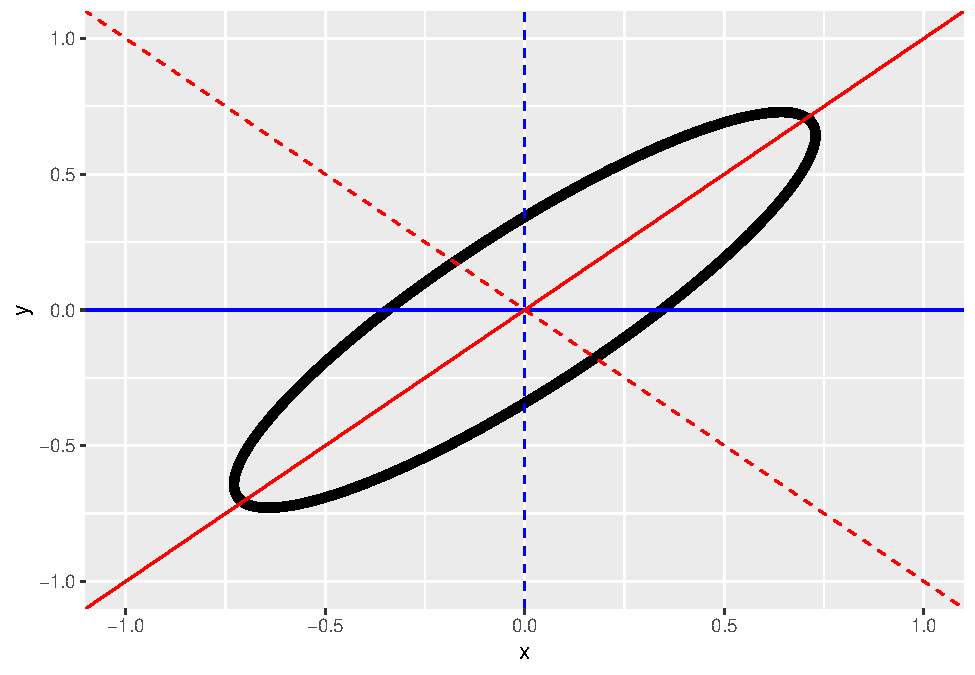
\includegraphics[width=0.5\linewidth]{supplementary_files/figure-latex/anisotropy-1} 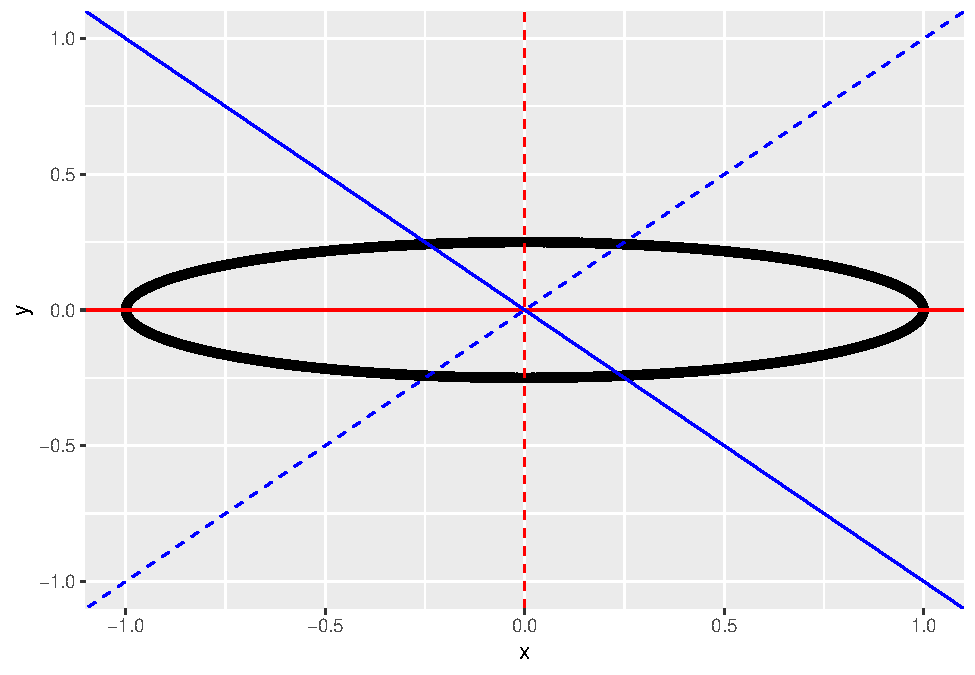
\includegraphics[width=0.5\linewidth]{supplementary_files/figure-latex/anisotropy-2} \caption{In the left figure, the ellipse of an isotropic spatial covariance function centered at the origin is shown. In the right figure, the ellipse of an anisotropic spatial covariance function centered at the origin is shown. The black outline of each ellipse is a level curve of equal correlation. }\label{fig:anisotropy}
\end{figure}

Figure\(~\)\ref{fig:anisotropy} shows ellipses for an isotropic and
anisotropic spatial covariance function centered at the origin (a
distance of zero). The black outline of each ellipse is a level curve of
equal correlation. The left ellipse (a circle) represents an isotropic
covariance function. The distance at which the correlation between two
observations lays on the level curve is the same in all directions. The
right ellipse represents an anisotropic covariance function. The
distance at which the correlation between two observations lays on the
level curve is different in different directions.

To accommodate spatial anisotropy, the original coordinates must be
transformed such that the transformed coordinates yield an isotropic
spatial covariance. This transformation involves a rotation and a
scaling. Consider a set of \(x\) and \(y\) coordinates that should be
transformed into \(x^*\) and \(y^*\) coordinates. This transformation is
formally defined as \begin{equation*}
  \begin{bmatrix}
    x^* \\
    y^*
  \end{bmatrix} = 
  \begin{bmatrix}
    1 & 0 \\
    0 & 1 / S
  \end{bmatrix}
  \begin{bmatrix}
    \cos(\alpha) & \sin(\alpha) \\
    -\sin(\alpha) & \cos(\alpha)
  \end{bmatrix}  
  \begin{bmatrix}
    x \\
    y
  \end{bmatrix}.
\end{equation*} The original coordinates are first multiplied by the
rotation matrix, which rotates the coordinates clockwise by angle
\(\alpha\). They are then multiplied by the scaling matrix, which scales
the minor axis of the spatial covariance ellipse by the reciprocal of
\(S\). The transformed coordinates are then used to compute distances
and the spatial covariances in Table\(~\)\ref{tab:cov_splm}. This type
of anisotropy is more formally known as ``geometric'' anisotropy because
it involves a geometric transformation of the coordinates.
Figure\(~\)\ref{fig:anisotropy2} shows this process step-by-step.

\begin{figure}
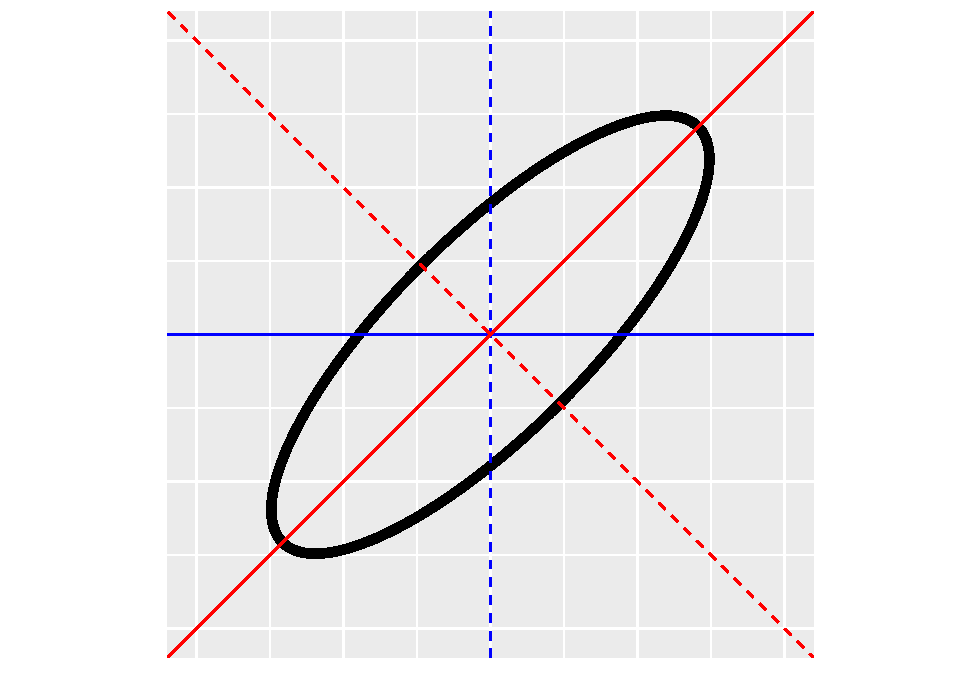
\includegraphics[width=0.33\linewidth]{supplementary_files/figure-latex/anisotropy2-1} 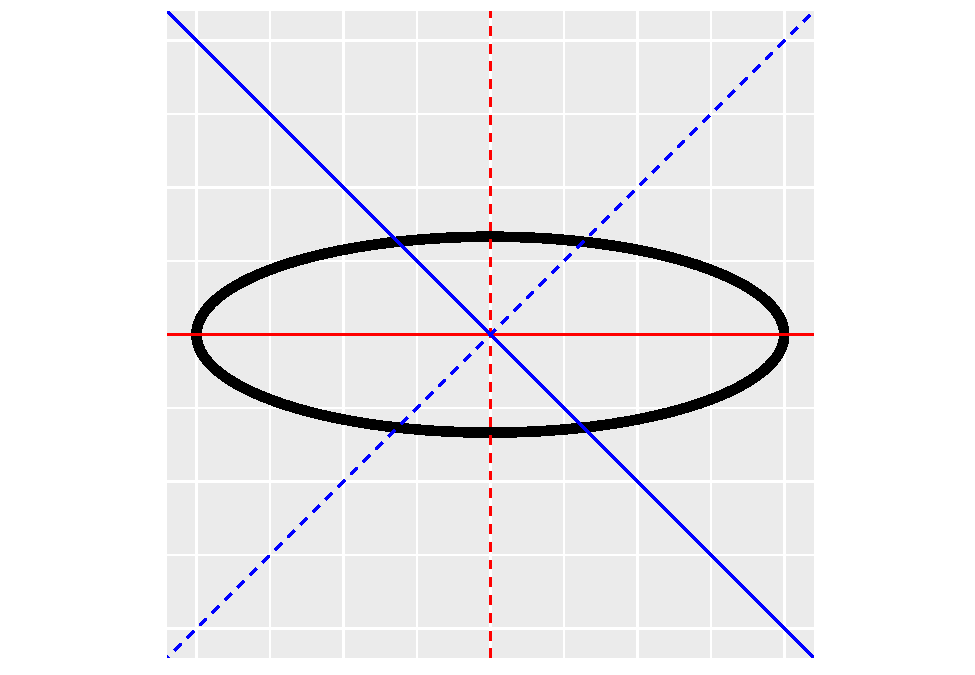
\includegraphics[width=0.33\linewidth]{supplementary_files/figure-latex/anisotropy2-2} 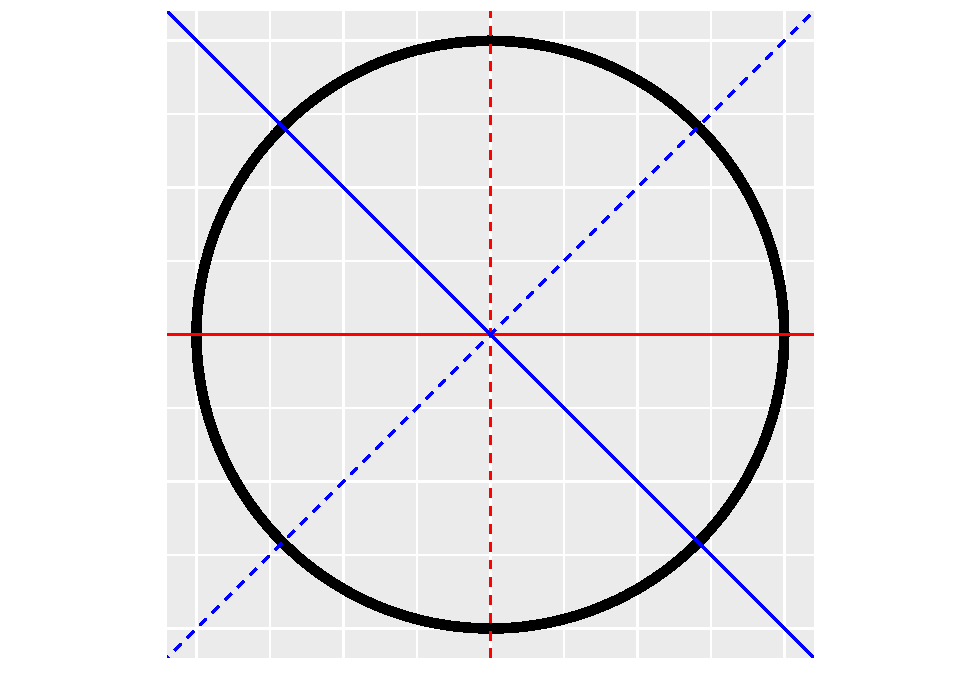
\includegraphics[width=0.33\linewidth]{supplementary_files/figure-latex/anisotropy2-3} \caption{In the left figure, the ellipse of an anisotropic spatial covariance function centered at the origin is shown. The blue lines represent the original axes and the red lines the transformed axes. The solid lines represent the x-axes and the dotted lines the y-axes. Note that the solid, red line is the major axis of the ellpise and the dashed, red line is the minor axis of the ellipse. In the center figure, the ellipse has been rotated clockwise by the rotate parameter so the major axis is the transformed x-axis and the minor axis is the transformed y-axis. In the right figure, the minor axis of the ellipse has been scaled by the reciprocal of the scale parameter so that the ellipse becomes a circle, which corresponds to an isotropic spatial covariance function. The transformed coordinates are then used to compute distances and spatial covariances.}\label{fig:anisotropy2}
\end{figure}

Anisotropy parameters (\(\alpha\) and \(S\)) can be estimated in
\texttt{spmodel} using restricted maximum likelihood or maximum
likelihood. Estimating anisotropy can be challenging. First, we need to
restrict the parameter space so that the two parameters are identifiable
(there is a unique parameter set for each possible outcome). We
restricted \(\alpha\) to \([0, \pi]\) radians due to symmetry of the
covariance ellipse at rotations \(\alpha\) and \(\alpha + j \pi\), where
\(j\) is any integer. We also restricted \(S\) to occur on \([0, 1]\)
because we have defined \(S\) as the scaling factor for the length of
the minor axis relative to the major axis -- otherwise it would not be
clear whether \(S\) refers to the minor or major axis. Given this
restricted parameter space, there is still an issue of local maxima,
particularly at rotation parameters near zero, which have a rotation
very close to rotation parameter \(\pi\), but zero is far from \(\pi\)
in the parameter space. To address the local maxima problem, each
optimization iteration actually involves two likelihood evaluations --
one for \(\alpha\) and another for \(|\pi - \alpha|\), where \(|\cdot|\)
denotes absolute value. Thus one likelihood evaluation is always in
\([0, \pi/2]\) radians and another in \([\pi/2, \pi]\) radians,
exploring different quadrants of the parameter space and allowing
optimization to test solutions near zero and \(\pi\) simultaneously.

Anisotropy parameters cannot be estimated in \texttt{spmodel} when
\texttt{estmethod} is \texttt{sv-wls} or \texttt{sv-cl}. However, known
anisotropy parameters for these estimation methods can be specified via
\texttt{spcov\_initial} and incorporated into estimation of
\(\boldsymbol{\theta}\) and \(\boldsymbol{\beta}\). Anisotropy is not
defined for areal data given its (binary) neighborhood structure.

\hypertarget{partition-factors}{%
\subsection{Partition Factors}\label{partition-factors}}

A partition factor is a factor (or categorical) variable in which
observations from different levels of the partition factor are assumed
uncorrelated. A partition matrix \(\mathbf{P}\) of dimension
\(n \times n\) can be constructed to represent the partition factor. The
\(ij\)th element of \(\mathbf{P}\) equals one if the observation in the
\(i\)th row and \(j\)th column are from the same level of the partition
factor and zero otherwise. Then the initial covariance matrix (ignoring
the partition factor) is updated by taking the Hadmard (element-wise)
product with the partition matrix: \begin{equation*}
 \boldsymbol{\Sigma}_{updated} = \boldsymbol{\Sigma}_{initial} \odot \mathbf{P},
\end{equation*} where \(\odot\) indicates the Hadmard product. Partition
factors impose a block structure in \(\boldsymbol{\Sigma}\), which
allows for efficient computation of \(\boldsymbol{\Sigma}^{-1}\) used
for estimation and prediction.

When computing the empirical semivariogram using \texttt{esv()},
semivariances are ignored when observations are from different levels of
the partition factor. For the \texttt{sv-wls} and \texttt{sv-cl}
estimation methods, semivariances are ignored when observations are from
different levels of the partition factor.

\hypertarget{subsec:bigdata}{%
\subsection{\texorpdfstring{Big Data (\texttt{splm()}
only)}{Big Data (splm() only)}}\label{subsec:bigdata}}

Big data model-fitting is accommodated in \texttt{spmodel} using a
``local indexing'' approach. Suppose there are \(m\) unique indexes, and
each observation is in one index. Then \(\boldsymbol{\Sigma}\) can be
represented blockwise as \begin{equation}\label{eq:full_cov}
  \boldsymbol{\Sigma} = 
  \begin{bmatrix}
  \boldsymbol{\Sigma}_{1,1} & \boldsymbol{\Sigma}_{1,2} & \hdots & \hdots & \boldsymbol{\Sigma}_{1,m} \\
  \boldsymbol{\Sigma}_{2,1} & \boldsymbol{\Sigma}_{2,2} & \boldsymbol{\Sigma}_{2,3} & \hdots & \boldsymbol{\Sigma}_{2,m} \\
  \vdots & \boldsymbol{\Sigma}_{3,2} & \ddots & \boldsymbol{\Sigma}_{3,4} & \vdots \\
  \vdots & \vdots & \boldsymbol{\Sigma}_{4,3} & \ddots & \vdots \\
  \boldsymbol{\Sigma}_{m,1} & \hdots & \hdots & \hdots & \boldsymbol{\Sigma}_{m, m}
  \end{bmatrix},
\end{equation} To perform estimation for big data, observations with the
same index value are assumed independent of observations with different
index values, yielding a ``big-data'' covariance matrix given by
\begin{equation}\label{eq:bd_cov}
  \boldsymbol{\Sigma}_{bd} = 
  \begin{bmatrix}
  \boldsymbol{\Sigma}_{1,1} & \boldsymbol{0} & \hdots & \hdots & \boldsymbol{0} \\
  \boldsymbol{0} & \boldsymbol{\Sigma}_{2,2} & \boldsymbol{0} & \hdots & \boldsymbol{0} \\
  \vdots & \boldsymbol{0} & \ddots & \boldsymbol{0} & \vdots \\
  \vdots & \vdots & \boldsymbol{0} & \ddots & \vdots \\
  \boldsymbol{0} & \hdots & \hdots & \hdots & \boldsymbol{\Sigma}_{m, m}
  \end{bmatrix},
\end{equation} Estimation then proceeds as described in
Section\(~\)\ref{subsec:estimation} using \(\boldsymbol{\Sigma}_{bd}\)
instead of \(\boldsymbol{\Sigma}\). When computing the empirical
semivariogram, semivariances are ignored when observations have
different local indexes. For the \texttt{sv-wls} and \texttt{sv-cl}
estimation methods, semivariances are ignored when observations have
different local indexes. Via Equation\(~\)\ref{eq:bd_cov}, it can be
seen that the local index acts as a partition factor separate from the
partition factor explicitly defined by \texttt{partition\_factor}.

spmodel allows for custom local indexes to be passed to \texttt{splm()}.
If a custom local index is not passed, the local index is determined
using the \texttt{"random"} or \texttt{"kmeans"} method. The
\texttt{"random"} method assigns observations to indexes randomly based
on the number of groups desired. The \texttt{"kmeans"} method uses
k-means clustering (MacQueen and others 1967) on the x-coordinates and
y-coordinates to assign observations to indexes (based on the number of
clusters (groups) desired).

The estimate of \(\boldsymbol{\beta}\) when using
Equation\(~\)\ref{eq:bd_cov} is given by
\begin{equation}\label{eq:beta_bd}
  \hat{\boldsymbol{\beta}}_{bd} = (\mathbf{X}^\top \boldsymbol{\hat{\Sigma}}^{-1}_{bd}\mathbf{X})^{-1}\mathbf{X}^\top \boldsymbol{\hat{\Sigma}}^{-1}_{bd} \mathbf{y} = \mathbf{T}^{-1}_{xx}\mathbf{t}_{xy},
\end{equation} where
\(\mathbf{T}_{xx} = \sum_{i = 1}^m \mathbf{X}_i^\top \boldsymbol{\hat{\Sigma}}^{-1}_{i, i}\mathbf{X}_i\)
and
\(\mathbf{t}_{xy} = \sum_{i = 1}^m \mathbf{X}_i^\top \hat{\boldsymbol{\Sigma}}^{-1}_{i, i} \mathbf{y}_i\).
Note that in \(\hat{\boldsymbol{\beta}}_{bd}\), \(\mathbf{X}_i\) and
\(\mathbf{y}_i\) are the subsets of \(\mathbf{X}\) and \(\mathbf{y}\),
respectively, for the \(i\)th local index. Equation\(~\)\ref{eq:beta_bd}
acts as a pooled estimator of \(\boldsymbol{\beta}\) across the indexes.

\texttt{spmodel} has four approaches for estimating the covariance
matrix of \(\hat{\boldsymbol{\beta}}_{bd}\). The choice is determined by
the \texttt{var\_adjust} argument to \texttt{local}. The first approach
is implements no adjustment (\texttt{var\_adjust\ =\ "none"}) and simply
uses \(\mathbf{T}_{xx}^{-1}\), which is the covariance matrix of
\(\hat{\boldsymbol{\beta}}_{bd}\) using \(\boldsymbol{\Sigma}_{bd}\)
(Equation\(~\)\ref{eq:bd_cov}). While computationally efficient, this
approach ignores the covariance across indexes. It can be shown that the
covariance of \(\hat{\boldsymbol{\beta}}_{bd}\) using
\(\boldsymbol{\Sigma}\) (Equation\(~\)\ref{eq:full_cov}) is given by
\begin{equation}\label{eq:var_theo}
  \mathbf{T}_{xx}^{-1} + \mathbf{T}_{xx}^{-1} \mathbf{W}_{xx}\mathbf{T}_{xx}^{-1},
\end{equation} where \begin{equation*}
\mathbf{W} = \sum_{i = 1}^{m - 1} \sum_{j = i + 1}^m (\mathbf{X}^\top \hat{\boldsymbol{\Sigma}}^{-1}_{i, i} \hat{\boldsymbol{\Sigma}}_{i, j} \hat{\boldsymbol{\Sigma}}^{-1}_{j, j} \mathbf{X}_j) + (\mathbf{X}^\top \hat{\boldsymbol{\Sigma}}^{-1}_{i, i} \hat{\boldsymbol{\Sigma}}_{i, j} \hat{\boldsymbol{\Sigma}}^{-1}_{j, j} \mathbf{X}_j)^\top
\end{equation*} Equation\(~\)\ref{eq:var_theo} can be viewed as the sum
of the unadjusted covariance matrix of \(\hat{\boldsymbol{\beta}}_{bd}\)
(\(\mathbf{T}_{xx}^{-1}\)) and a correction that incorporates the
covariance across indexes
(\(\mathbf{T}_{xx}^{-1} \mathbf{W}_{xx}\mathbf{T}_{xx}^{-1}\)). This
adjustment is known as the ``theoretically-correct''
(\texttt{var\_adjust\ =\ "theoretical"}) adjustment because it uses
\(\boldsymbol{\Sigma}\). The theoretical adjustment is the default
adjustment in \texttt{spmodel} because it is theoretically correct, but
it is the most computationally expensive adjustment. Two alternative
adjustments are also provided, and while not equal to the theoretical
adjustment, they are easier to compute. They are the empirical
(\texttt{var\_adjust\ =\ "empirical"}) and pooled
(\texttt{var\_adjust\ =\ "pooled"}) adjustments. The empirical
adjustment is given by \begin{equation*}
\frac{1}{m(m -1)} \sum_{i = 1}^m (\boldsymbol{\hat{\beta}}_i - \boldsymbol{\hat{\beta}}_{bd})(\boldsymbol{\hat{\beta}}_i - \boldsymbol{\hat{\beta}}_{bd})^\top,
\end{equation*} where
\(\boldsymbol{\hat{\beta}}_i = (\mathbf{X}^\top \hat{\boldsymbol{\Sigma}}^{-1} \mathbf{X})^{-1}\mathbf{X}_i^\top \hat{\boldsymbol{\Sigma}}^{-1}_{i, i} \mathbf{y}_i\).
A similar adjustment could use
\(\boldsymbol{\hat{\beta}}_i = (\mathbf{X}_i^\top \hat{\boldsymbol{\Sigma}}^{-1}_{i, i} \mathbf{X}_i)^{-1}\mathbf{X}_i \hat{\boldsymbol{\Sigma}}^{-1}_{i, i} \mathbf{y}_i\),
which more closely resembles a composite likelihood approach. This
approach is sensitive to the presence of at least one singularity in
\(\mathbf{X}_i^\top \hat{\boldsymbol{\Sigma}}^{-1}_{i, i} \mathbf{X}_i\),
in which case the variance adjustment cannot be computed. The
\texttt{"pooled"} variance adjustment is given by \begin{equation*}
\frac{1}{m^2} \sum_{i = 1}^m (\mathbf{X}^\top_i \hat{\boldsymbol{\Sigma}}^{-1}_{i, i} \mathbf{X}_i)^{-1}.
\end{equation*} Note that the pooled variance adjustment cannot be
computed if any
\(\mathbf{X}_i^\top \hat{\boldsymbol{\Sigma}}^{-1}_{i, i} \mathbf{X}_i\)
are singular.

\hypertarget{sec:sprnorm}{%
\section{\texorpdfstring{\texttt{sprnorm()}}{sprnorm()}}\label{sec:sprnorm}}

Spatial normal (Gaussian) random variables are simulated by taking the
sum of a fixed mean and random errors. The random errors have mean zero
and covariance matrix \(\boldsymbol{\Sigma}\). A realization of the
random errors is obtained from \(\boldsymbol{\Sigma}^{1/2} \mathbf{e}\),
where \(\mathbf{e}\) is a normal random variable with mean zero and
covariance matrix \(\mathbf{I}\). Then the spatial normal random
variable equals \begin{equation*}
 \mathbf{y} = \boldsymbol{\mu} + \boldsymbol{\Sigma}^{1/2} \mathbf{e},
\end{equation*} where \(\boldsymbol{\mu}\) is the fixed mean. It follows
that \begin{equation*}
  \begin{split}
  \text{E}(\mathbf{y}) & = \boldsymbol{\mu} + \boldsymbol{\Sigma}^{1/2} \text{E}(\mathbf{e}) = \boldsymbol{\mu} \\
  \text{Cov}(\mathbf{y}) & = \text{Cov}(\boldsymbol{\Sigma}^{1/2} \mathbf{e}) = \boldsymbol{\Sigma}^{1/2} \text{Cov}(\mathbf{e}) \boldsymbol{\Sigma}^{1/2} = \boldsymbol{\Sigma}^{1/2} \boldsymbol{\Sigma}^{1/2} = \boldsymbol{\Sigma}
  \end{split}
\end{equation*}

\hypertarget{sec:vcov}{%
\section{\texorpdfstring{\texttt{vcov()}}{vcov()}}\label{sec:vcov}}

\texttt{vcov()} returns the variance-covariance matrix of estimated
parameters. Currently, \texttt{vcov()} only returns the
variance-covariance matrix of \(\hat{\boldsymbol{\beta}}\), the fixed
effects. The variance-covariance matrix of the fixed effects is given by
\((\mathbf{X}^\top \hat{\boldsymbol{\Sigma}}^{-1} \mathbf{X})^{-1}\).

\hypertarget{sec:iprod}{%
\section{A Note on Covariance Square Roots and Inverse
Products}\label{sec:iprod}}

Often \(\boldsymbol{\Sigma}^{-1}\) is not strictly needed for
estimation, prediction, or other purposes, but at least the product
between \(\boldsymbol{\Sigma}^{-1}\) and some other matrix is needed.
Consider the example of the covariance matrix of
\(\hat{\boldsymbol{\beta}}\) and observe
\(\mathbf{X}^\top \boldsymbol{\Sigma}^{-1} \mathbf{X}\) is needed. The
most direct way to find this product is certainly to obtain
\(\boldsymbol{\Sigma}^{-1}\) and then multiply by \(\mathbf{X}^\top\) on
the left and \(\mathbf{X}\) on the right. This is both computationally
expensive and cannot be used to compute products that involve
\(\boldsymbol{\Sigma}^{-1/2}\), which are often useful
(Section\(~\)\ref{sec:residuals}). It is helpful to rewrite
\(\mathbf{X}^\top \boldsymbol{\Sigma}^{-1} \mathbf{X}\) as
\(\mathbf{X}^\top (\mathbf{S}^\top)^{-1} \mathbf{S}^{-1} \mathbf{X} = (\mathbf{S}^{-1} \mathbf{X})^\top \mathbf{S}^{-1} \mathbf{X}\).
Then one computes the inverse products by finding \(\mathbf{S}\).

One way to find \(\mathbf{S}\) is to use an eigendecomposition. The
eigendecomposition of \(\boldsymbol{\Sigma}\) (which is real and
symmetric) is given by \begin{equation*}
\boldsymbol{\Sigma} = \mathbf{U} \mathbf{D} \mathbf{U}^\top,
\end{equation*} where \(\mathbf{U}\) is an orthogonal matrix of
eigenvectors of \(\boldsymbol{\Sigma}\) and \(\mathbf{D}\) is a diagonal
matrix with eigenvalues of \(\boldsymbol{\Sigma}\) on the diagonal. Then
\(\boldsymbol{\Sigma}^{1/2} = \mathbf{U} \mathbf{D}^{1/2} \mathbf{U}^\top\),
where \(\mathbf{D}^{1/2}\) is a diagonal matrix with square roots of
eigenvalues of \(\boldsymbol{\Sigma}\) on the diagonal. This result
follows because \(\mathbf{U}\) being orthogonal implies
\(\mathbf{U}^\top = \mathbf{U}^{-1}\) and \begin{equation*}
\boldsymbol{\Sigma}^{1/2}\boldsymbol{\Sigma}^{1/2} = \mathbf{U} \mathbf{D}^{1/2} \mathbf{U}^\top \mathbf{U} \mathbf{D}^{1/2} \mathbf{U}^\top = \mathbf{U} \mathbf{D}^{1/2} (\mathbf{U}^\top \mathbf{U}) \mathbf{D}^{1/2} \mathbf{U}^\top = \mathbf{U} \mathbf{D} \mathbf{U}^\top = \boldsymbol{\Sigma}.
\end{equation*} So then taking \(\mathbf{S} = \mathbf{D}^{1/2}\) implies
\(\mathbf{S}^{-1} = \mathbf{D}^{-1/2}\), which is straightforward to
calculate as \(\mathbf{D}^{1/2}\) is diagonal. So not only does the
eigendecomposition approach give us the inverse products, it also gives
us \(\boldsymbol{\Sigma}^{1/2}\) and \(\boldsymbol{\Sigma}^{-1/2}\).
While straightforward, this approach is less efficient than the Cholesky
decomposition (Golub and Van Loan 2013), which we discuss next.

The Cholesky decomposition decomposes \(\boldsymbol{\Sigma}\) into the
product between \(\mathbf{C}\) and \(\mathbf{C}^\top\)
(\(\boldsymbol{\Sigma} = \mathbf{C}\mathbf{C}^\top\)), where
\(\mathbf{C}\) is a lower triangular matrix. Note that \(\mathbf{C}\) is
generally not equal to \(\boldsymbol{\Sigma}^{1/2}\). Taking
\(\mathbf{S}\) to be \(\mathbf{C}\), we see that finding the inverse
products requires solving \(\mathbf{C}^{-1}\mathbf{X}\). Observe that
\(\mathbf{C}^{-1}\mathbf{X} = \mathbf{A}\) for some matrix
\(\mathbf{A}\). This implies \(\mathbf{X} = \mathbf{C}\mathbf{A}\),
which for \(\mathbf{A}\) can be efficiently solved using forward
substitution because \(\mathbf{C}\) is lower triangular.

The products in this document that involve \(\boldsymbol{\Sigma}^{1/2}\)
and \(\boldsymbol{\Sigma}^{-1/2}\) are actually implemented in
\texttt{spmodel} using \(\mathbf{C}\) and \(\mathbf{C}^{-1}\) (instead
of \(\boldsymbol{\Sigma}^{1/2}\) and \(\boldsymbol{\Sigma}^{-1/2}\)).
They are written in this document using \(\boldsymbol{\Sigma}^{1/2}\)
and \(\boldsymbol{\Sigma}^{-1/2}\) because the underlying concepts are
easier to communicate using square root notation.

\hypertarget{references}{%
\section*{References}\label{references}}
\addcontentsline{toc}{section}{References}

\hypertarget{refs}{}
\leavevmode\hypertarget{ref-brent1971algorithm}{}%
Brent, Richard P. 1971. ``An Algorithm with Guaranteed Convergence for
Finding a Zero of a Function.'' \emph{The Computer Journal} 14 (4):
422--25.

\leavevmode\hypertarget{ref-cook1979influential}{}%
Cook, R Dennis. 1979. ``Influential Observations in Linear Regression.''
\emph{Journal of the American Statistical Association} 74 (365):
169--74.

\leavevmode\hypertarget{ref-cook1982residuals}{}%
Cook, R Dennis, and Sanford Weisberg. 1982. \emph{Residuals and
Influence in Regression}. New York: Chapman; Hall.

\leavevmode\hypertarget{ref-cressie1985fitting}{}%
Cressie, Noel. 1985. ``Fitting Variogram Models by Weighted Least
Squares.'' \emph{Journal of the International Association for
Mathematical Geology} 17 (5): 563--86.

\leavevmode\hypertarget{ref-cressie1993statistics}{}%
---------. 1993. \emph{Statistics for Spatial Data}. John Wiley \& Sons.

\leavevmode\hypertarget{ref-curriero1999composite}{}%
Curriero, Frank C, and Subhash Lele. 1999. ``A Composite Likelihood
Approach to Semivariogram Estimation.'' \emph{Journal of Agricultural,
Biological, and Environmental Statistics}, 9--28.

\leavevmode\hypertarget{ref-goldman2000statistical}{}%
Goldman, Nick, and Simon Whelan. 2000. ``Statistical Tests of
Gamma-Distributed Rate Heterogeneity in Models of Sequence Evolution in
Phylogenetics.'' \emph{Molecular Biology and Evolution} 17 (6): 975--78.

\leavevmode\hypertarget{ref-golub2013matrix}{}%
Golub, Gene H, and Charles F Van Loan. 2013. \emph{Matrix Computations}.
JHU press.

\leavevmode\hypertarget{ref-harville1977maximum}{}%
Harville, David A. 1977. ``Maximum Likelihood Approaches to Variance
Component Estimation and to Related Problems.'' \emph{Journal of the
American Statistical Association} 72 (358): 320--38.

\leavevmode\hypertarget{ref-harville1992mean}{}%
Harville, David A, and Daniel R Jeske. 1992. ``Mean Squared Error of
Estimation or Prediction Under a General Linear Model.'' \emph{Journal
of the American Statistical Association} 87 (419): 724--31.

\leavevmode\hypertarget{ref-henderson1975best}{}%
Henderson, Charles R. 1975. ``Best Linear Unbiased Estimation and
Prediction Under a Selection Model.'' \emph{Biometrics}, 423--47.

\leavevmode\hypertarget{ref-hoeting2006model}{}%
Hoeting, Jennifer A, Richard A Davis, Andrew A Merton, and Sandra E
Thompson. 2006. ``Model Selection for Geostatistical Models.''
\emph{Ecological Applications} 16 (1): 87--98.

\leavevmode\hypertarget{ref-hrong1996approximate}{}%
Hrong-Tai Fai, Alex, and Paul L Cornelius. 1996. ``Approximate F-Tests
of Multiple Degree of Freedom Hypotheses in Generalized Least Squares
Analyses of Unbalanced Split-Plot Experiments.'' \emph{Journal of
Statistical Computation and Simulation} 54 (4): 363--78.

\leavevmode\hypertarget{ref-kackar1984approximations}{}%
Kackar, Raghu N, and David A Harville. 1984. ``Approximations for
Standard Errors of Estimators of Fixed and Random Effects in Mixed
Linear Models.'' \emph{Journal of the American Statistical Association}
79 (388): 853--62.

\leavevmode\hypertarget{ref-kenward1997small}{}%
Kenward, Michael G, and James H Roger. 1997. ``Small Sample Inference
for Fixed Effects from Restricted Maximum Likelihood.''
\emph{Biometrics}, 983--97.

\leavevmode\hypertarget{ref-kenward2009improved}{}%
---------. 2009. ``An Improved Approximation to the Precision of Fixed
Effects from Restricted Maximum Likelihood.'' \emph{Computational
Statistics \& Data Analysis} 53 (7): 2583--95.

\leavevmode\hypertarget{ref-littell2006sas}{}%
Littell, Ramon C, George A Milliken, Walter W Stroup, Russell D
Wolfinger, and Schabenberber Oliver. 2006. \emph{SAS for Mixed Models}.
SAS publishing.

\leavevmode\hypertarget{ref-macqueen1967some}{}%
MacQueen, James, and others. 1967. ``Some Methods for Classification and
Analysis of Multivariate Observations.'' In \emph{Proceedings of the
Fifth Berkeley Symposium on Mathematical Statistics and Probability},
1:281--97. 14. Oakland, CA, USA.

\leavevmode\hypertarget{ref-montgomery2021introduction}{}%
Montgomery, Douglas C, Elizabeth A Peck, and G Geoffrey Vining. 2021.
\emph{Introduction to Linear Regression Analysis}. John Wiley \& Sons.

\leavevmode\hypertarget{ref-myers2012generalized}{}%
Myers, Raymond H, Douglas C Montgomery, G Geoffrey Vining, and Timothy J
Robinson. 2012. \emph{Generalized Linear Models: With Applications in
Engineering and the Sciences}. John Wiley \& Sons.

\leavevmode\hypertarget{ref-nelder1965simplex}{}%
Nelder, John A, and Roger Mead. 1965. ``A Simplex Method for Function
Minimization.'' \emph{The Computer Journal} 7 (4): 308--13.

\leavevmode\hypertarget{ref-patterson1971recovery}{}%
Patterson, H Desmond, and Robin Thompson. 1971. ``Recovery of
Inter-Block Information When Block Sizes Are Unequal.''
\emph{Biometrika} 58 (3): 545--54.

\leavevmode\hypertarget{ref-pinheiro2006mixed}{}%
Pinheiro, José, and Douglas Bates. 2006. \emph{Mixed-Effects Models in S
and S-Plus}. Springer science \& business media.

\leavevmode\hypertarget{ref-prasad1990estimation}{}%
Prasad, NG Narasimha, and Jon NK Rao. 1990. ``The Estimation of the Mean
Squared Error of Small-Area Estimators.'' \emph{Journal of the American
Statistical Association} 85 (409): 163--71.

\leavevmode\hypertarget{ref-satterthwaite1946approximate}{}%
Satterthwaite, Franklin E. 1946. ``An Approximate Distribution of
Estimates of Variance Components.'' \emph{Biometrics Bulletin} 2 (6):
110--14.

\leavevmode\hypertarget{ref-schluchter1990small}{}%
Schluchter, Mark D, and Janet T Elashoff. 1990. ``Small-Sample
Adjustments to Tests with Unbalanced Repeated Measures Assuming Several
Covariance Structures.'' \emph{Journal of Statistical Computation and
Simulation} 37 (1-2): 69--87.

\leavevmode\hypertarget{ref-searle2009variance}{}%
Searle, Shayle R, George Casella, and Charles E McCulloch. 2009.
\emph{Variance Components}. John Wiley \& Sons.

\leavevmode\hypertarget{ref-self1987asymptotic}{}%
Self, Steven G, and Kung-Yee Liang. 1987. ``Asymptotic Properties of
Maximum Likelihood Estimators and Likelihood Ratio Tests Under
Nonstandard Conditions.'' \emph{Journal of the American Statistical
Association} 82 (398): 605--10.

\leavevmode\hypertarget{ref-stram1994variance}{}%
Stram, Daniel O, and Jae Won Lee. 1994. ``Variance Components Testing in
the Longitudinal Mixed Effects Model.'' \emph{Biometrics}, 1171--7.

\leavevmode\hypertarget{ref-wolf1978helmert}{}%
Wolf, Helmut. 1978. ``The Helmert Block Method-Its Origin and
Development.'' In \emph{Proceedings of the Second International
Symposium on Problems Related to the Redefinition of North American
Geodetic Networks,(NOAA, Arlington-Va, 1978)}, 319--26.

\leavevmode\hypertarget{ref-wolfinger1994computing}{}%
Wolfinger, Russ, Randy Tobias, and John Sall. 1994. ``Computing Gaussian
Likelihoods and Their Derivatives for General Linear Mixed Models.''
\emph{SIAM Journal on Scientific Computing} 15 (6): 1294--1310.

\bibliographystyle{unsrt}
\bibliography{references.bib}


\end{document}
